\documentclass[chapterprefix=true, 11pt, a4paper, oneside, parskip=half, listof=totoc, bibliography=totoc, numbers=noendperiod]{scrbook}

% \documentclass[chapterprefix=true, 11pt, a4paper, oneside, parskip=half, bibliography=totoc, numbers=noendperiod]{scrbook} % Verzeichnisse nicht in ToC

\usepackage{lmodern}
\usepackage[utf8]{inputenc}
\usepackage[T1]{fontenc}
\usepackage[bottom=32mm,left=25mm,right=25mm]{geometry}
\usepackage[onehalfspacing]{setspace}
\usepackage[stretch=10]{microtype}
\usepackage{xcolor}
\usepackage{titling}
\usepackage{listings}
\usepackage{minted}
\usepackage{graphicx}
\usepackage{hyperref}
\usepackage[ngerman]{babel}
\usepackage{csquotes}
\usepackage[style=alphabetic, backend=biber, bibencoding=utf8, sorting=ynt]{biblatex}
\usepackage[toc, acronym]{glossaries}
\usepackage[onehalfspacing]{setspace}
\usepackage[stretch=10]{microtype}
\usepackage{imakeidx}
\usepackage{caption}
\usepackage{subcaption}
\usepackage{amssymb}
\usepackage{amsmath}
\usepackage[automark,headsepline]{scrlayer-scrpage}



\addbibresource{references/images.bib}
\addbibresource{references/online.bib}
\addbibresource{references/repos.bib}
\addbibresource{references/scientific.bib}

\makenoidxglossaries

\renewcommand{\lstlistlistingname}{Quellcodeverzeichniss}
\renewcommand{\lstlistingname}{Code snippet}

\setminted{xleftmargin=20pt,linenos,breaklines,fontsize=\footnotesize}

\newglossarystyle{dottedlocations}{%
	\glossarystyle{list}%
	\renewcommand*{\glossaryentryfield}[5]{%
		\item[\glsentryitem{##1}\glstarget{##1}{##2}] \emph{##3}%
		\unskip\leaders\hbox to 2.9mm{\hss.}\hfill##5}%
	\renewcommand*{\glsgroupskip}{}%
}

\loadglsentries{glossary.tex}

\definecolor{danger}{RGB}{220, 53, 69}
\newenvironment{longlisting}{\captionsetup{type=listing}}{}
\newcommand*{\gradeType}[1]{\gdef\thegradetype{#1}}
\newcommand*{\firstExaminer}[1]{\gdef\thefirstexaminer{#1}}
\newcommand*{\secondExaminer}[1]{\gdef\thesecondexaminer{#1}}
\newcommand*{\matrikelnr}[1]{\gdef\thematrikelnr{#1}}
\newcommand*{\submitDate}[1]{\gdef\thesubmitdate{#1}}

\def\changemargin#1#2{\list{}{\rightmargin#2\leftmargin#1}\item[]}
\let\endchangemargin=\endlist

\renewcommand*{\maketitle}{
	\begin{titlepage}
		\begin{changemargin}{-0.5cm}{0.0cm}
		\begin{figure}[H]
			\centering
			
\includegraphics[width=0.5\textwidth]{resources/title/Q01_HTW_Berlin_Logo_quer_pos_FARBIG_CMYK.eps}
		\end{figure}
		\begin{center}
			\vfill
			{\Large \thetitle\par}
			\vskip 0.5cm
			{\large \bfseries Abschlussarbeit\par}
			\vskip 0.5cm
			{\large zur Erlangung des akademischen Grades\vskip 0.5cm \bfseries \thegradetype}
			\vskip 0.5cm
			{\large an der}
			\vskip 0.5cm
			{\large Hochschule für Technik und Wirtschaft Berlin}
			\vskip 0.0cm
			{\large Fachbereich IV: Informatik, Kommunikation und Wirtschaft}
			\vskip 0.0cm
			{\large Studiengang Angewandte Informatik}
			\vfill
			\begin{flushleft}
				\begin{tabular}[t]{rl}
					1. Prüfer:                  & \thefirstexaminer  \\
					2. Prüfer:                  & \thesecondexaminer \\
					\\
					Eingereicht von:            & \theauthor \\
					Immatrikulationsnummer:     & \thematrikelnr \\
					Eingereicht am:             & \thesubmitdate
				\end{tabular}
			\end{flushleft}
		\end{center}
		\end{changemargin}
	\end{titlepage}
}

\title{Untersuchungen von Style Transfer Methoden für die Verwendung mit leistungsarmer Hardware}
\author{Christoph Stach}
\matrikelnr{0555912}
\submitDate{28.08.2018}
\firstExaminer{Prof. Dr. Christin Schmidt}
\secondExaminer{Patrick Baumann}
\gradeType{Bachelor of Science (B.Sc.)}

\begin{document}

\maketitle

\pagenumbering{gobble}
\chapter*{Danksagung}

Ich danke allen Personen, die mich bei der Erstellung dieser Abschlussarbeit unterstützt haben. Besonderer Dank gilt meinen Eltern, Annegret Stach und Rüdiger Stach sowie meiner Schwester Pauline Stach, die mich während der gesamten Zeit meines Studiums unterstützt haben.

Weitere Danksagungen gehen an meine Freunde und meine Betreuer Frau Prof. Dr. Christin Schmidt und Herrn Patrick Baumann, die mir bei der Erstellung dieser Arbeit mit Rat und technischen Ressourcen zur Seite standen.

\pagebreak

\chapter*{Abstract}

Die Abschlussarbeit im Bereich der angewandten Informatik handelt davon, verschiedene Style Transfer Methoden zu implementieren, die Konzepte zu verstehen und sie auf Tauglichkeit für Systeme mit leistungsarmer Hardware zu testen. Style Transfer ist ein Bereich des Deep Learning. Es werden zwei oder mehrere willkürliche Bilder zu einem neuen Bild kombiniert. Beim ersten Bild wird der Inhalt aus dem Bild herausgefiltert, z.B. aus einem Foto, auf dem ein Vogel zu sehen ist. Aus dem zweiten Bild wird der Stil herausgefiltert, z.B. aus einem abstrakt gezeichneten Gemälde. Das Ergebnis ist die Mischung aus Objekt und Stil. Die Ausrichtung, ob das Ergebnis mehr Objekt oder eher Stil ist, kann durch Parameter beeinflusst werden. Es werden unterschiedliche Algorithmen sowie ihre Hyperparameter untersucht. Anschließend wird ihre Performanz gemessen und die Ergebnisse miteinander verglichen. \clearpage

\pagenumbering{roman}
\tableofcontents
\listoffigures
\listoftables
\lstlistoflistings

\newpage
\pagenumbering{arabic}
\chapter{Einleitung}

Im Kapitel Einleitung wird die Idee und persönliche Motivation, Zielsetzung und Vorgehensweise und genereller Aufbau der Arbeit beschrieben.

\section{Idee und Motivation}

Die Idee einen Algorithmus für Neural Style Transfer zu entwickeln der auf Geräten mit leistungsarmer Hardware funktioniert, entstand durch mein persönliches 
Intresse an der Webentwicklung und an Machine Learning Verfahren. Bereits vor dem Studium an der HTW Berlin konnte ich Erfahrungen im Bereich der Webentwicklung/Frontend Entwicklung sammeln und habe bereits professionell in diesem Bereich gearbeitet. Im Rahmen des Hochschulstudiums lernte ich
Verfahren um Machine- und Deep Learning anzwenden. Besonders der Bereich Computervision war dabei für mich intressant. Ich nutze die Bachelorarbeit dazu diese beiden Intressengebiete zu kombinieren und möchte erforschen wie es möglich ist Style Transfer Methoden auf Geräten mit leistungsarmer Hardware auszuführen.

Style Transfer ist ein intressantes Forschungsobjekt und erfordert die intensive Auseinandersetzung mit Convolutional Neural Networks \cite{lecun-gradientbased-learning-applied-1998} und dem Backpropagation Algorithmus \cite{doi:10.1162/neco.1989.1.4.541}. Außerdem müssen benutzerdefinierte Loss-Functions, die nicht in Problemstellungen der Bildklassifizierung verwendet werden, benutzt werden.

\section{Zielsetzung}

Ziel des Projektes ist ein Softwaresystem zu erstellen, das in der Lage ist, Style Transfer auf Geräten mit leistungsarmer Hardware zu ermöglichen. Dabei sollen Mechanismen des Style Transfer untersucht werden und sukzessiv verbessert werden.

\section{Vorgehensweise und Aufbau der Arbeit}

Nach der Einarbeitung in die Grundlagen von Style Transfer \cite{DBLP:journals/corr/GatysEB15a, DBLP:journals/corr/JohnsonAL16} Methoden, müssen entsprechende Algorithmen gefunden werden. Da es sich um die Manipulation von Bildern handelt, werden Convolutional Neural Networks \cite{lecun-gradientbased-learning-applied-1998} zum Einsatz kommen, die sich dazu eignen, Features aus Bildern zu extrahieren. Im nächsten Schritt muss ein Datensatz wie ImageNet \cite{imagenet_cvpr09} oder Coco \cite{DBLP:journals/corr/LinMBHPRDZ14} benutzt oder in entsprechender Größe generiert werden, mit dem ein solches Netzwerk trainiert werden kann. Letztendlich muss das Netzwerk auf den verwendeten Datensatz durch Backpropagation \cite{doi:10.1162/neco.1989.1.4.541} optimiert werden. Die Implementierung des Models in den Prototypen eines Softwaresystems soll der Veranschaulichung der Ergebnisse dienen.

Abschließend werden umfangereiche Experimente mit verschiedenen Einstellungen und Netzwerkarchitekturen durchgeführt.
Die Ergebnisse werden verglichen, in einem Fazit kritisch betrachtet und eine Schlussfolgerungen gezogen. \clearpage
\chapter{Grundlagen}
\label{cha:fundamentals}

Im Kapitel Grundlagen werden die erfordentlichen Grundlagen erleutert, die notwendig sind um die Funktionsweise von Style Transfer zu verstehen. Außerdem wird auf bestehende Arbeiten in diesem Bereich eingegangen.

\section{Feedforward Neural Network}

Feedforward Neural Networks werden im Bereich des Deep Learning eingesetzt. Dabei werden unteschiedliche Arten von Layern zu einem Neuronalen Netzwerk zusammen gesetzt. Je nach Aufgabenstellung sind unteschiedliche Arten von Layer-Kombination sinnvoll.

Ein Feedforward Neural Network definiert eine Abildung von $ y = f(x; \phi) $ wobei $ \phi $ (auch mit $ w $ notiert) Gewichtungsparameter des Netzwerk sind. Es wird Feedforward genannt, da die Informationen $ x $ von vorne nach hinten durch die einzelnen Layer des Networks fließen und am Ende $ y $ ausgeben. Die Layer des Netzwerk sind dabei wiederum Unterfunktionen die in einer Kettenstruktur ineinander übergehen. Bei einem Neuronalen Netzwerk mit den drei Layern $ f^{(1)} $, $ f^{(2)} $, $ f^{(2)} $ ergibt sich der Aufbau $ f(x) = f^{(3)}(f^{(2)}(f^{(1)}(x))) $. Der erste Layer eines Netzwerks nennt sich Input-Layer, der letzte Output-Layer. Alle zwischenliegenden Layer werden Hidden-Layer genannt. Je mehr Layer ein Netzwerk besitzt, desto komplexere mathematische Funktionen kann es abbilden und desto tiefer ist es. Daher rührt auch Name Deep Neural Network und Deep Learning \cite[164-165]{Goodfellow-et-al-2016}.

\pagebreak

\section{Fully-Connected Neural Network}

Fully-Connected Neural Networks bestehen aus mehreren hintereinander geschalteten Fully-Connected-Layern. Der Name rührt daraus, dass zwischen zwei aufeinanderfolgenden Layern alle Neuronen miteinander verbunden sind.

\begin{figure}[H]
	\centering
	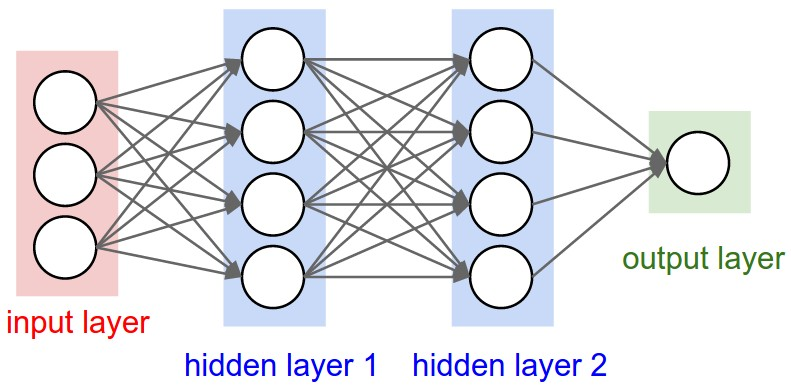
\includegraphics[width=0.95\textwidth]{resources/content/fully_connected.jpg}
	\caption{Fully-Connected Neural Network \cite{fully_connected_img}}
	\label{img:fully_connected}
\end{figure}

Die Kreise stellen die Neuronen dar und die Kanten sind die Gewichtungsfaktoren.
Eine solche Struktur kann mit einer mit einer einziger Matrix-Multiplation berechnet werden.

\begin{align}
	f(x) = \sigma(x * w + b)
\end{align}

In der Formel steht $ x $ für die Eingangsdaten, $ w $ für die Gewichtungsfaktoren, $ b $ für einen Biaswert. Letztlich läuft das berechnete Ergebniss durch eine Aktivierungsfunktion $ \sigma $, die nachfolgend in \ref{sec:activation_functions} beschrieben wird.

Ausgehend von einem Neuronalen Netzwerk mit einem Input-Layer mit zwei Neuronen, einem Hidden-Layer mit drei Neuronen, einem Output-Layer mit einem Neuron, einer Minibatchgröße von drei und der Aktvierungsfunktion $ \sigma(x) = {\begin{cases}0&{\text{if }}x<0\\x&{\text{if }}x\geq 0\end{cases}} $ ergibt sich folgendes Beispiel:

\begin{equation}
	\vspace{5pt}
	x = \begin{pmatrix} 
		0.0 & 0.0 \\
		1.0 & 1.0 \\ 
		2.0 & 2.0
	\end{pmatrix}
	\vspace{5pt}
	w_{1} = \begin{pmatrix} 
		1.0 & 1.0 \\
		1.0 & 1.0 \\ 
		0.5 & 0.5
	\end{pmatrix}
	\vspace{5pt}
	w_{2} = \begin{pmatrix} 
		1.0 \\
		1.0 \\ 
		0.5
	\end{pmatrix}
\end{equation}

Die Werte der letzten Zeilen in den Gewichtsmatrizen $ w_{1} $ und $ w_{2} $ sind die Gewichtungsfaktoren für den Bias-Wert. Den Eingabedaten $ x $ wird vor Durchlauf durch einen Layer ein fester Wert (Bias) von $ 1 $ hinzugefügt. Nach Durchlauf durch den ersten Layer ergibt sich dementsprechend folgendes Zwischenergebnis:

\begin{equation}
	\sigma \left(
	\begin{pmatrix} 
		0.0 & 0.0 & 1.0 \\
		1.0 & 1.0 & 1.0 \\ 
		2.0 & 2.0 & 1.0
	\end{pmatrix} 
	\times
	\begin{pmatrix} 
		1.0 & 1.0 \\
		1.0 & 1.0 \\ 
		0.5 & 0.5
	\end{pmatrix}
	\right)
	= 
	\begin{pmatrix} 
		0.5 & 0.5 \\
		2.5 & 2.5 \\ 
		4.5 & 4.5
	\end{pmatrix}
\end{equation}

Wiederholt wird dieser Vorgang mit der Gewichtsmatrix $ w_{2} $ des zweiten Layers:

\begin{equation}
	\sigma \left(
	\begin{pmatrix} 
		0.5 & 0.5 & 1.0 \\
		2.5 & 2.5 & 1.0 \\ 
		4.5 & 4.5 & 1.0
	\end{pmatrix}
	\times
	\begin{pmatrix} 
		1.0 \\
		1.0 \\ 
		0.5
	\end{pmatrix}
	\right)
	= 
	\begin{pmatrix} 
		1.5 \\
		5.5 \\ 
		9.5
	\end{pmatrix}
\end{equation}

\section{Aktivierungsfunktionen}
\label{sec:activation_functions}

Die im voherigen Beispiel verwendete Aktivierungsfunktion nennt sich ReLU \cite{Nair:2010:RLU:3104322.3104425}.

\begin{figure}[H]
	\centering
	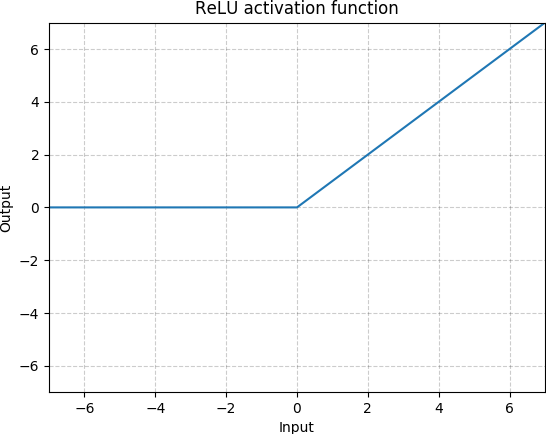
\includegraphics[width=0.50\textwidth]{resources/content/ReLU.png}
	\caption{ReLU-Aktivierungsfunktion \cite{relu_activation_function_img}}
	\label{img:relu_activation_function}
\end{figure}


Neben der ReLU-Aktivierungsfunktion existieren weitere Aktiverungsfunktionen, die im Zusammenhang mit Neuronalen Netzwerken verwendet werden.
Im Folgende werden die in dieser Arbeit verwendeten Aktivierungsfunktionen beschrieben.

\subsection{LeakyReLU, PReLU}

Die Aktiverungsfunktionen LeakyReLU und PReLU sind Abwandulung von ReLU und werden um den Parameter $ \alpha $ ergänzt. Bei LeakyReLU handelt es sich bei $ \alpha $ um einen fixen, einstellbaren Wert und bei PReLU wird dieser im Laufe der Trainingsphase gelernt \cite{DBLP:journals/corr/XuWCL15}.

\begin{equation}
	\sigma(\alpha ,x) = {
		\begin{cases}
			\alpha x & {\text{if }} x < 0 \\
			x        & {\text{if }} x \geq 0
		\end{cases}
	}
\end{equation}

Visualisiert besitzen beide Aktiverungsfunktionen folgende Form:

\begin{figure}[H]
	\centering
	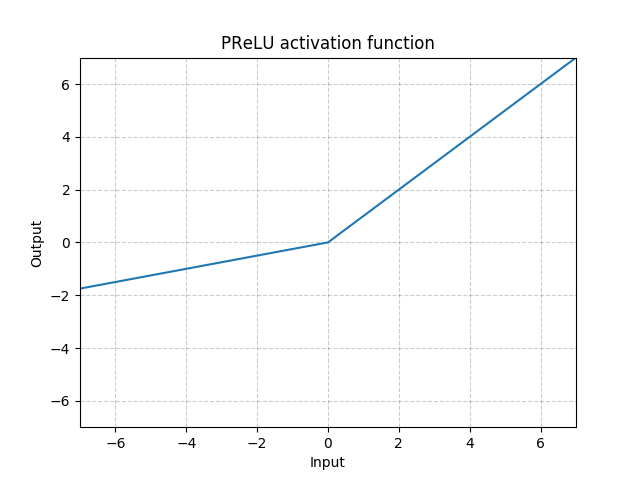
\includegraphics[width=0.50\textwidth]{resources/content/PReLU.png}
	\caption{LeakyReLU-, PReLU-Aktivierungsfunktion \cite{prelu_activation_function_img}}
	\label{img:prelu_activation_function}
\end{figure}

\subsection{Hardtanh}
\label{sec:hardtanh}

Die Hardtanh Funktion wird in dieser Arbeit als abschliesende Aktiverungsfunktion genutzt \cite{DBLP:journals/corr/abs-1811-03378, Collobert:2011:NLP:1953048.2078186}.

\begin{equation}
	\sigma(x) = {
		\begin{cases}
			1  & {\text{if }} x > 1 \\ 
			-1 & {\text{if }} x < -1 \\
			x  & {\text{otherwise}}
		\end{cases}
	 }
\end{equation}

\pagebreak

Sie ist in der Lage die Ergebnisse auf einen festgelegten Bereich zu beschränken.

\begin{figure}[H]
	\centering
	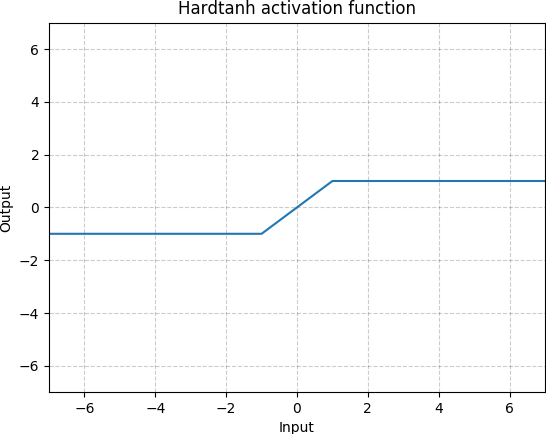
\includegraphics[width=0.55\textwidth]{resources/content/Hardtanh.png}
	\caption{Hardtanh-Aktivierungsfunktion \cite{hardtanh_activation_function_img}}
	\label{img:hardtanh_activation_function}
\end{figure}

\subsection{Sigmoid}
\label{sec:sigmoid}

Die Sigmoid-Funktion wird in dieser Arbeit als alternative, abschliesende Aktiverungsfunktion genutzt \cite{DBLP:journals/corr/abs-1811-03378}.

\begin{equation}
	\sigma(x) = \frac{ 1 } { 
		1 + e^{ -x }
	}
\end{equation}

Die Ergebnisse der Sigmoid-Funktion konvergieren zu 0 und 1 ereichen diese jedoch nie komplett.

\begin{figure}[H]
	\centering
	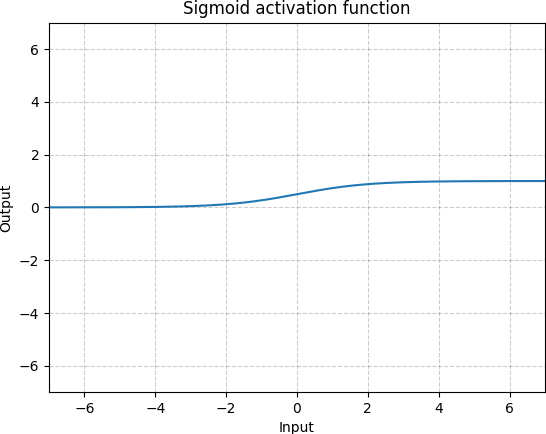
\includegraphics[width=0.55\textwidth]{resources/content/Sigmoid.png}
	\caption{Sigmoid-Aktivierungsfunktion \cite{sigmoid_activation_function_img}}
	\label{img:sigmoid_activation_function}
\end{figure}

\section{Convolutional Neural Network}
\label{sec:conv_networks}

Ein Convolutional Neural Network, auch CNN genannt, besteht aus mehreren aufeinanderfolgenden Convolutional-Layern, sowie
abschließend beliebig vielen Fully-Connected-Layern (siehe \ref{img:cnn_example_network}). Convolutional-Layer dienen der Featureextraktion. Die Fully-Connected-Layer sind für die Klassifizierung zuständig. Nachfolgend wird das Prinzip einer Convolution (zu dt. Faltung) erleutert.

\begin{figure}[H]
	\centering
	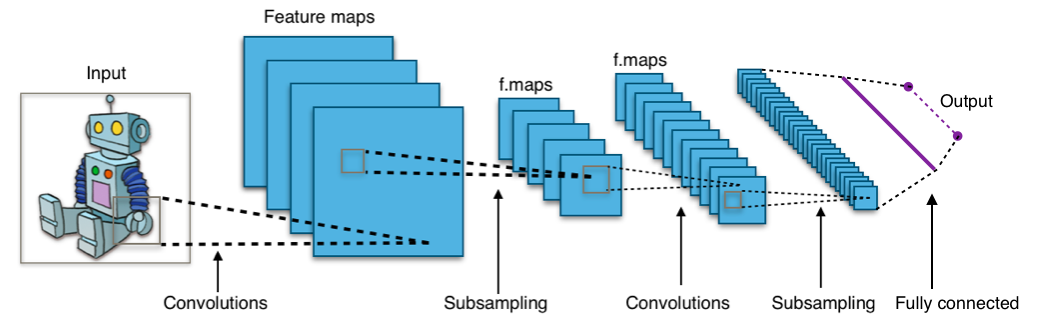
\includegraphics[width=0.95\textwidth]{resources/content/cnn/typical_cnn.png}
	\caption{Beispiel CNN Architektur \cite{typical_cnn_img}}
	\label{img:cnn_example_network}
\end{figure}

Ein Convolutional-Layer akzeptiert Daten in Form eines Bildes $ I $ in den Dimensionen $ W_1 \times H_1 \times C_1 $. Optional wird das Bild mit $ P $ Nullen an den Rändern aufgefüllt. Über das Bild fahren $ N $ Filter der Größe $ F $ mit einer Schrittweite $ S $ und führen an jeder Stelle ein Skalarprodukt mit den Daten der Bildmatrix durch. Daraus ergibt sich eine neue Matrix mit den Dimensionen $ W_2 \times H_2 \times C_2 $:

\begin{itemize}
	\item $ W_2 = (W_1 - F) / S + 1 $
	\item $ H_2 = (H_1 - F) / S + 1 $
	\item $ C_2 = N $
\end{itemize}

\begin{figure}[H]
	\centering
	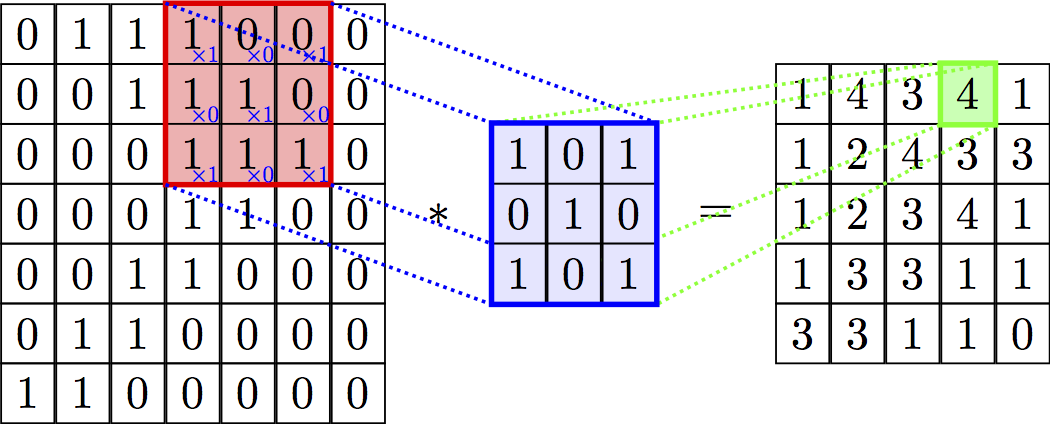
\includegraphics[width=0.90\textwidth]{resources/content/cnn/convolution_croped.png}
	\caption{Berechnungsschritt während einer Convolution \cite{convolution_img}}
	\label{img:convolution_img}
\end{figure}

Die Ergebnisse nach Durchlauf eines Convolutional-Layer werden Feature Maps oder \gls{activation_map}s genannt. Im trainierten CNN erkennen frühe Convolutional-Layer Kanten, Kurven und feine Muster. Spätere Layer erkennen komplette geometrische Figuren bis hin zu komplexen Mustern sowie Schemen von reellen Objekten und Gegenständen.

\section{Backprogation}
\label{sec:backpropagation}

Um ein Neuronales Netzwerk zu trainieren muss das Loss, welches ein Neurales Netzwerk erzeugt, minimiert werden. Das Loss berechnet sich aus der Differenz zwischen $ y $ und $ \hat{y} $. Wobei $ y $ die echten gelabelten Ergebnisse sind und $ \hat{y} $ die Vorhersage, die das Neuronale Netzwerk erzeugt.
Anhand dieser Daten kann ein Optimizer, wie beispielsweise \gls{adam} \cite{kingma2015adam}, die Gewichte des Netzwerks anpassen um das Loss zu minimieren.

\begin{figure}[H]
	\centering
	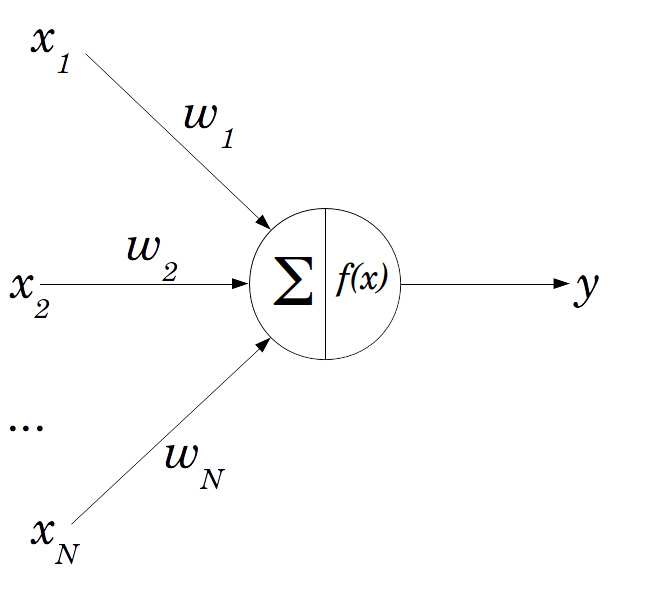
\includegraphics[width=0.4\textwidth]{resources/content/perceptron.png}
	\caption{Visualisierung eines Neurons (auch Perceptron \cite{80230} genannt) \cite{perceptron_img}}
	\label{img:perceptron_img}
\end{figure}

Als Beispiel diehnt die mathematische Funktion eines 2-dimensionalen Neurons mit angehängter Sigmoid-Aktivierungsfunktion. Dabei werden die Eingabewerte durch die Variable $ x $ und die Gewichte des Neurons durch die Variable $ w $ beschrieben.

\begin{align}
	f(w, x) = \frac{1}{ 1 + e^{ - (w_{0}x_{0} + w_{1}x_{1} + w_{2}) } }
\end{align}

\pagebreak

Folgender Graph veranschaulicht die Berechnung der Gradienten der Funktion.

% https://drive.google.com/file/d/18BC0RLOulbBQSE5Oddg1pVNL9UrhQLx0/view?usp=sharing
\begin{figure}[H]
	\centering
	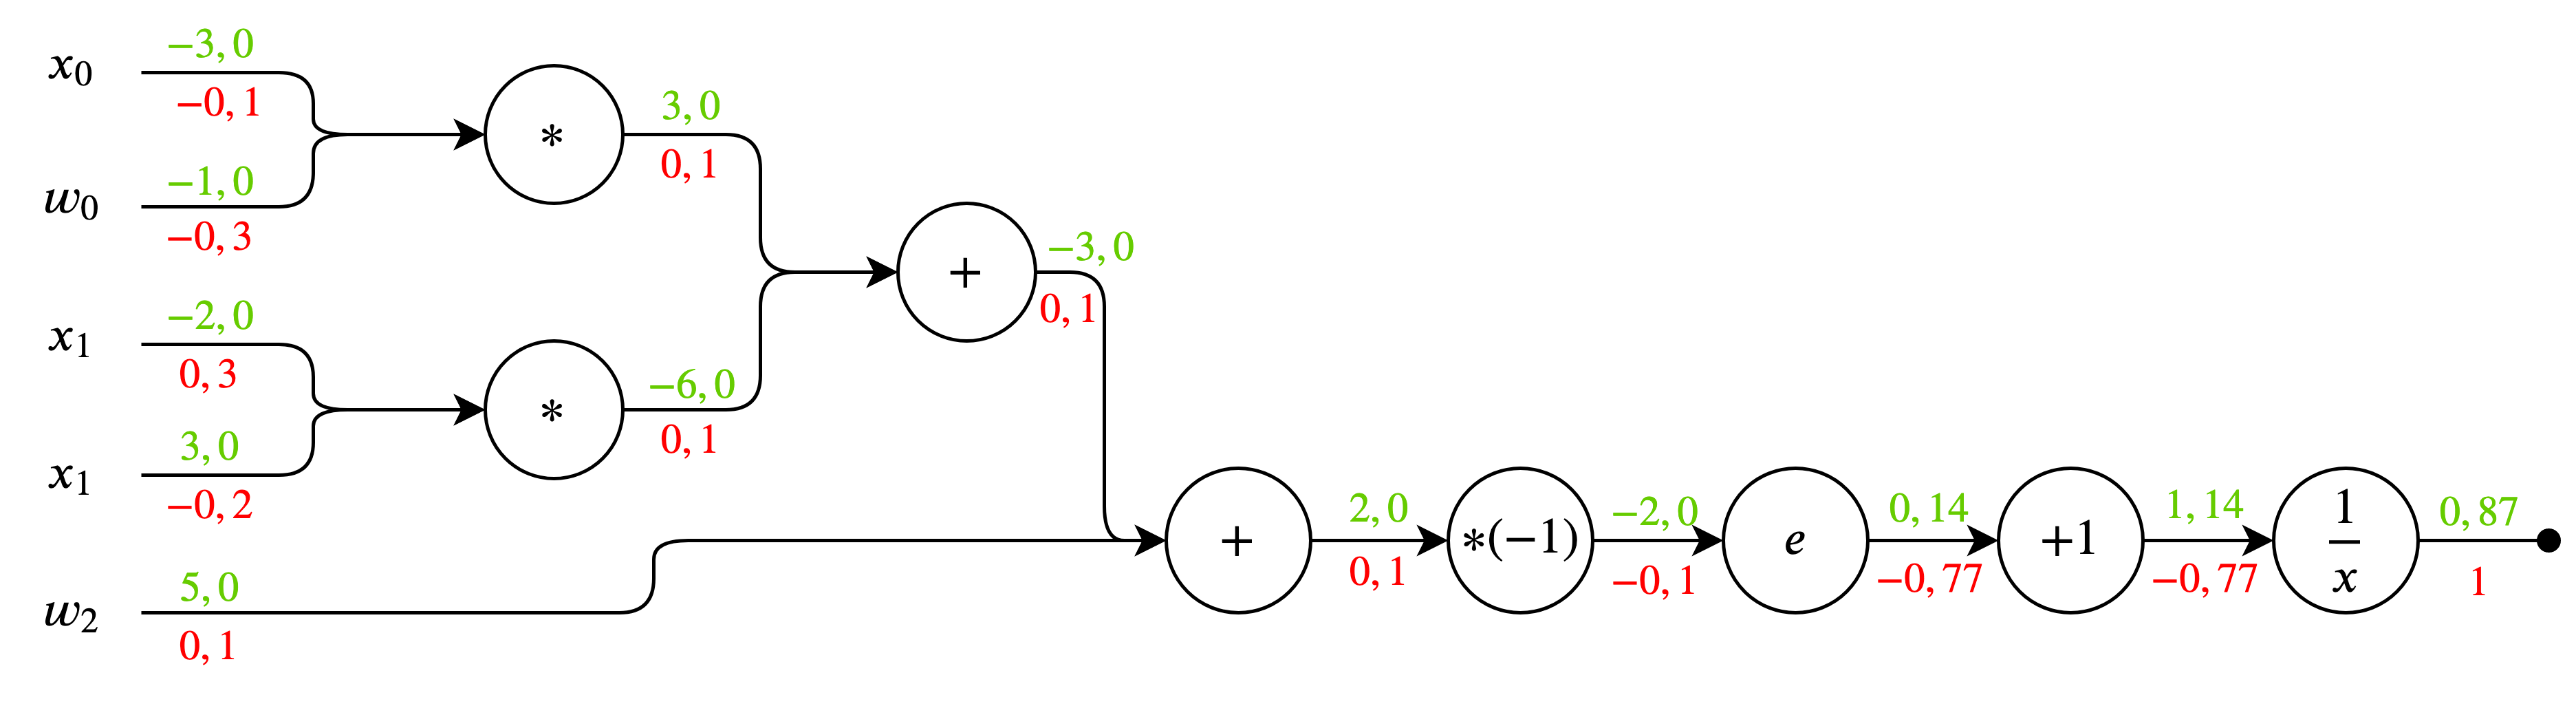
\includegraphics[width=1\textwidth]{resources/content/backpropagation.png}
	\caption{Forward-Pass in Grün und Backward-Pass in Rot dargestellt \cite{cs231n2}}
	\label{img:backpropagation_img}
\end{figure}

Die Funktion wird in beliebig viele Unterfunktionen zerteilt und in Form eines gerichteten Graphen aufgeschrieben.
In einem Forward-Pass werden die Zwischenergebnisse (hier in Grün dargestellt) oberhalb der Kanten festgehalten.

Im Backward-Pass (Zwischenergebnisse in Rot dargestellt) wird von jedem Knoten die erste Ableitung gebildet. Die Zwischenergebnisse des Forward-Pass werden in die Ableitung eingesetzt und danach mit dem Backward-Passergebnis des Vorschritts multipliziert.

Beispielrechnungen des Backward-Pass der letzten drei Knoten: 

\begin{align}
	& f(x) = \frac{1}{x} \rightarrow \frac{\partial f}{\partial x} = \frac{-1}{ x^{2} }
	& -0,77 \approx 1 * \frac{-1}{ 1,14^{2} }
\end{align}

\begin{align}
	& f(x) = x + 1 \rightarrow \frac{\partial f}{\partial x} = 1
	& -0,77 = -0,77 * 1
\end{align}

\begin{align}
	& f(x) = e^{x} \rightarrow \frac{\partial f}{\partial x} = e^{x}
	& -0,1 \approx -0,77 * e^{-2}
\end{align}

Durch die Berechnung der Gradienten der Gewichtsvariable $ w $ ist der Optimizer in der Lage $ w $ Schritt für Schritt anzupassen und somit das Loss verringern.

\pagebreak

\section{Verwandte Arbeiten}

Diese Arbeit basiert größtenteils auf den bereits bestehenden Lösungen von Johnson et. al. und Gatys et al., welche in den folgenden Abschnitten erklärt werden.

\subsection{Neural Style Transfer}
\label{sec:neural_style_transfer}

Hierbei handelt sich um eine Technik um den Stil von artistischen Bildern auf ein anderes willkürliches Bild zu übertragen.
Das Verfahren nutzt dabei einen optimisierenden Ansatz. Dabei werden die Pixel eines Eingangsbildes Schritt für Schritt den Pixeln 
des gewünschten Ausgangsbildes angepasst. 

Der Neural Style Transfer Algorithmus, beschrieben im Paper \cite{DBLP:journals/corr/GatysEB15a}, optimiert direkt die Pixel eines Bildes anhand einem sogenannten Perceptual-Loss. Die entsprechende Loss-Funktion besteht aus mehreren Teilen. Einem Content-Loss und einem Style-Loss. Optional kann zusätztlich ein Total-Variation-Loss verwendet werden. Das gesammte Perceptual-Loss wird über Hyperparameter konfiguriert, welche die Gewichtung der Unterfunktionen auf das Gesamt-Loss wiederspiegeln.

Content-Loss und Style-Loss benutzen dabei ein bereits auf einem großen Datensatz vortrainiertes Model. In dieser Arbeit wird das VGG16-Model \cite{DBLP:journals/corr/SimonyanZ14a} verwendet. Das Content-Loss vergleicht Features eines Inhaltsbildes mit den Features des Ausgangsbild. Das Style-Loss vergleicht Features eines Stilbildes mit den Features des Ausgangsbildes.

\begin{figure}[H]
	\centering
	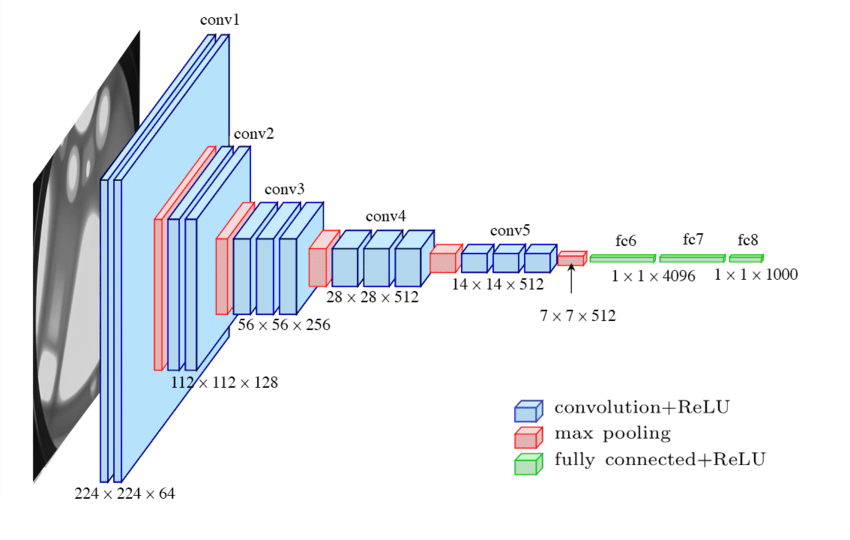
\includegraphics[width=0.70\textwidth]{resources/content/vgg16.png}
	\caption{Architektur des VGG16-Netzwerks \cite{vgg16_img}}
	\label{img:vgg16_img}
\end{figure}

\subsubsection{Content-Loss}
\label{sec:content_loss}

Um das Content-Loss zu berechnen wird nicht direkt das Contentbild mit dem Ausgangsbild verglichen, stattdessen werden die \gls{activation_map}s nach bestimmten Layern im VGG16-Netzwerk (auch Loss-Network genannt) verwendet. Auch ist es möglich die \gls{activation_map}s mehrerer Layer zu benutzen, da unterschiedliche Layer ein anderes \gls{receptive_field} haben und somit unterscheidliche Informationen speichern.

\begin{figure}[H]
	\centering
	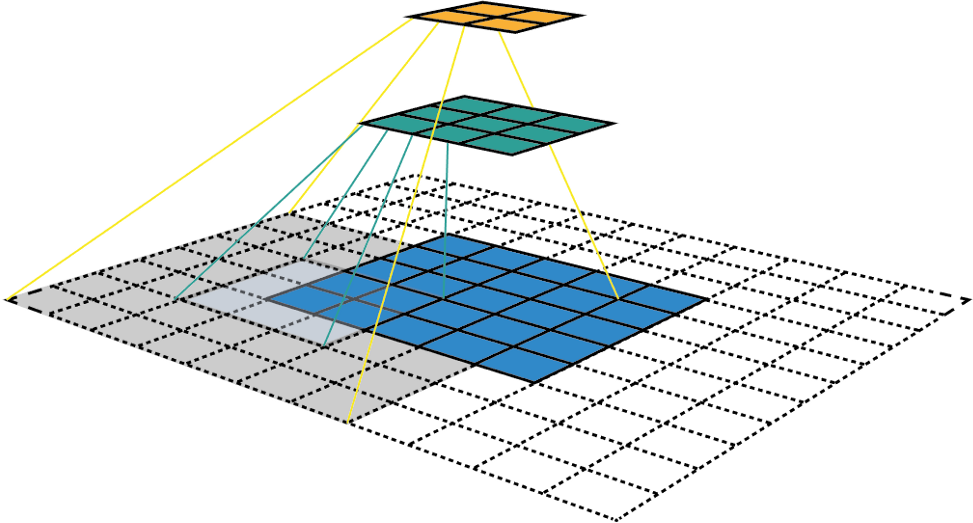
\includegraphics[width=0.79\textwidth]{resources/content/receptive_field.png}
	\caption{Visualisierung des \gls{receptive_field} über drei CNN-Layer \cite{receptive_field_img}}
	\label{img:receptive_field_img}
\end{figure}

Zwischen den \gls{activation_map}s $ P $  des Contentbildes $ \vec{p} $ und den \gls{activation_map}s $ F $ des generierten Bildes $ \vec{x} $ wird das \gls{mse_loss} anhand der gegebenen Layer $ l $ berechnet.

\begin{equation}
	\label{eq:content_loss}
    L_{content} ( \vec{p}, \vec{x}, l ) = \frac{1}{2} \sum_{i, j} (F_{ij}^{l} - P_{ij}^{l})^2
\end{equation}

\subsubsection{Style-Loss}
\label{sec:style_loss}

Das Style-Loss verwendet die \gls{activation_map}s nicht direkt sondern bildet vorher die Gram-Matrix dieser. Das hat zur Folge das räumliche Informationen verworfen werden, jedoch Farben und Muster erhalten bleiben, die beim Übertragen des Stils die wichtigste Rolle einehmen.

Um die Gram-Matrix mehrerer \gls{activation_map}s zu berechnen, werden die Matrizen geflächt, Height- und Width-Dimension werden zu einer Dimension zusammengefügt. Daraus ergibt sich eine 2-dimensionale Matrix der Form $ C \times HW $. Diese wird transponiert mit sich selbst multipliziert.

\begin{equation}
	\label{eq:gram_matrix_1}
	G_{ij}^{l} = \sum_{k} F_{ik}^{l} F_{jk}^{l}
\end{equation}

Es wird die Gram-Matrix, $ G $ aus dem Stilbild und $ A $ aus dem generierten Bild, anhand der gebenen Layer $ l $ berechnet, anschließend normalisiert und das \gls{mse_loss} gebildet.

\begin{equation}
	\label{eq:gram_matrix_2}
	E_{l} = \frac{1}{4N_{l}^{2} M_{l}^2} = \sum_{i, j} ( G_{ij}^{l} - A_{ij}^{l} )^2
\end{equation}

Das Style-Loss ergibt sich aus der gewichteten Summe der Layer-Losses.

\begin{equation}
	\label{eq:style_loss}
	L_{style} ( \vec{a}, \vec{x} ) = \sum_{l=0}^{L} w_{l} E_{l}
\end{equation}

\subsubsection{Total-Variation-Loss}
\label{sec:total_variation_Loss}

Bei der Total-Variation-Loss-Funktion handelt es sich um einen Signal-Denoising-Algorithmus \cite{RUDIN1992259, DBLP:journals/corr/EstrelaMS16}. Sie sorgt dafür das die Pixel der generierten Bilder sanft in einander überlaufen. Farblich sehr unterschiedliche, nah aneinanderliegende Pixel erzeugen ein hohes Loss. So können Verpixelungseffekte vermieden werden. Sie kann optional eingesetzt werden um das Resultat der generierten Bilder zu verbessern.

\begin{equation}
	\label{eq:total_variation_loss}
	L_{tv} ( \vec{x} ) = \sum_{i,j} | y_{i + 1, j} - y_{i, j} | + | y_{i, j + 1} - y_{i,j} |
\end{equation}

\subsubsection{Perceptual-Loss}
\label{sec:perceptual_loss}

Das Perceptual-Loss ist die Kombination aus Content-, Style- und Total-Variation-Loss und wird um die Parameter $ \alpha $, $ \beta $ und $ \gamma $ ergänzt, mit denen die Gewichtung der Losses eingestellt wird.

\begin{equation}
	\label{eq:perceptual_loss}
    L_{perceptual} ( \vec{p}, \vec{a}, \vec{x} ) = \alpha L_{content} ( \vec{p}, \vec{x} ) + \beta L_{style} ( \vec{a}, \vec{x} ) + \gamma L_{tv} ( \vec{x} )
\end{equation}

\subsection{Fast Neural Style Transfer}
\label{sec:fast_neural_style_transfer}

Im Gegensatz zum im Kapitel \ref{sec:neural_style_transfer} vorgestellten Algorithmus, in dem die Pixel des Eingangsbildes direkt optimiert werden, wird ein
Neuronales Netzwerk darauf trainiert, die Konzepte eines Stils zu erlernen. Dieses Verfahren wird im Paper \cite{DBLP:journals/corr/JohnsonAL16} genauer beschrieben. Pro Style wird dabei ein Model trainiert. Die verwendete Loss-Funktion ist das bereits zuvor beschriebene Perceptual-Loss \ref{sec:perceptual_loss}.

\begin{figure}[H]
	\centering
	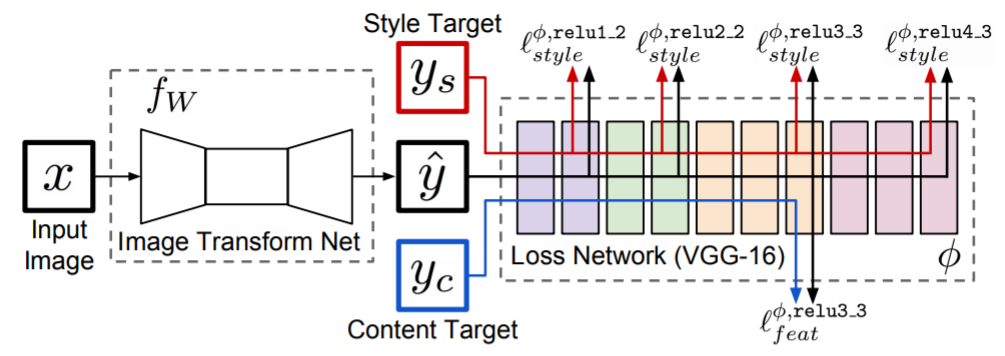
\includegraphics[width=0.79\textwidth]{resources/content/fast_neural_style.png}
	\caption{Trainingsprozess eines Image Transformer Networks \cite{DBLP:journals/corr/JohnsonAL16}}
	\label{img:fast_neural_style_transfer}
\end{figure}

Durch die Verwendung eines Image Transformer Networks kann die Berechnungszeit verbessert werden, da das neu gestylte Bild mit einem Forward-Pass durch das Netzwerk erstellt wird. Die rechenintensive Optimierung durch den Backpropagation-Algorithmus \ref{sec:backpropagation} entfällt. Das Training eines Image Transformer Netzworks nimmt jedoch viel Zeit in Anspruch. \clearpage
\chapter{Methodologie}
\label{cha:methodology}

Im Kapitel Methodologie wird das allgemeine Vorgehen beschrieben, dass notwendig ist, um die in Kapitel \ref{cha:fundamentals} vorgestellten Algorithmen zu implementieren.

\section{Vorherige Arbeiten}

Bereits vor Erstellung dieser Arbeit gab es Ansätze, den Neural Style Transfer zu realisieren. Diese Arbeit orientiert sich an den bereits bestehenden Entwicklungen und versucht diese zu verbessern sowie auf Geräten mit leistungsarmer Hardware zu testen. Im GIT-Repository von Justin Johnson \cite{Johnson2015} ist der Neural Style Transfer \ref{sec:neural_style_transfer} auf Basis des Papers \cite{DBLP:journals/corr/GatysEB15a} mit dem Framework Torch \cite{torch} implementiert. Außerdem existiert ein online Toturial des Frameworks PyTorch \cite{OnlineToturialNeuralStylePyTorch}.

Der Fast Neural Style Transfer \ref{sec:fast_neural_style_transfer} orientiert sich ebenfalls an einem GIT-Repository von Justin Johnson \cite{Johnson2016}, dass den Algorithmus im Framework Torch implementiert. Des weiteren ist er als Beispielalgorithmus im PyTorch GIT-Repository \cite{PyTorchFastNeuralStyle} vorhanden.

Neben den vorgestellten Implementierungen existieren viele weitere Implementierungen in unterschiedlichen Frameworks verschiedener Autoren sowie entsprechende Blogeinträge auf beispielsweise \url{https://towardsdatascience.com/}.

\pagebreak

\section{Neural Style Transfer}
\label{sec:method_neural_style_transfer}

Als erster Schritt wird die Loss-Funktion entwickelt. Da das Loss aus drei Teilen besteht, eignet es sich, dieses als Klasse zu realisieren. Style-Loss, Content-Loss sowie Total-Variation-Loss können als einzelne Methoden dieser Klasse implementiert werden und als Gesamt-Loss mit Gewichtung zusammengefasst werden. Außerdem können die notwendigen Hyperparameter des Perceptual-Loss der Klasse bei Instanziierung übergeben werden. Des weiteren werden unterschiedliche Hilfsfunktionen benötigt, um die Gram-Matrix zu berechnen sowie das Laden und Speichern von Bildern und deren Umwandlung in und von \gls{tensor}en\footnote{Als \gls{tensor}en werden Matrizen/Vektoren jeglicher Dimensionen bezeichnet} zu ermöglichen.

Um mathematische Operationen durchzuführen, die bei Berechnung der Gram-Matrix oder des Loss verwendet werden, benötigt man außerdem unterschiedliche Funktionen, die das Rechnen mit Vektoren und Matrizen ermöglichen.


% https://drive.google.com/file/d/1gn8Q9fPT6ZOsA8DkEg-lpwexMV28C-Px/view?usp=sharing
\begin{figure}[H]
	\centering
	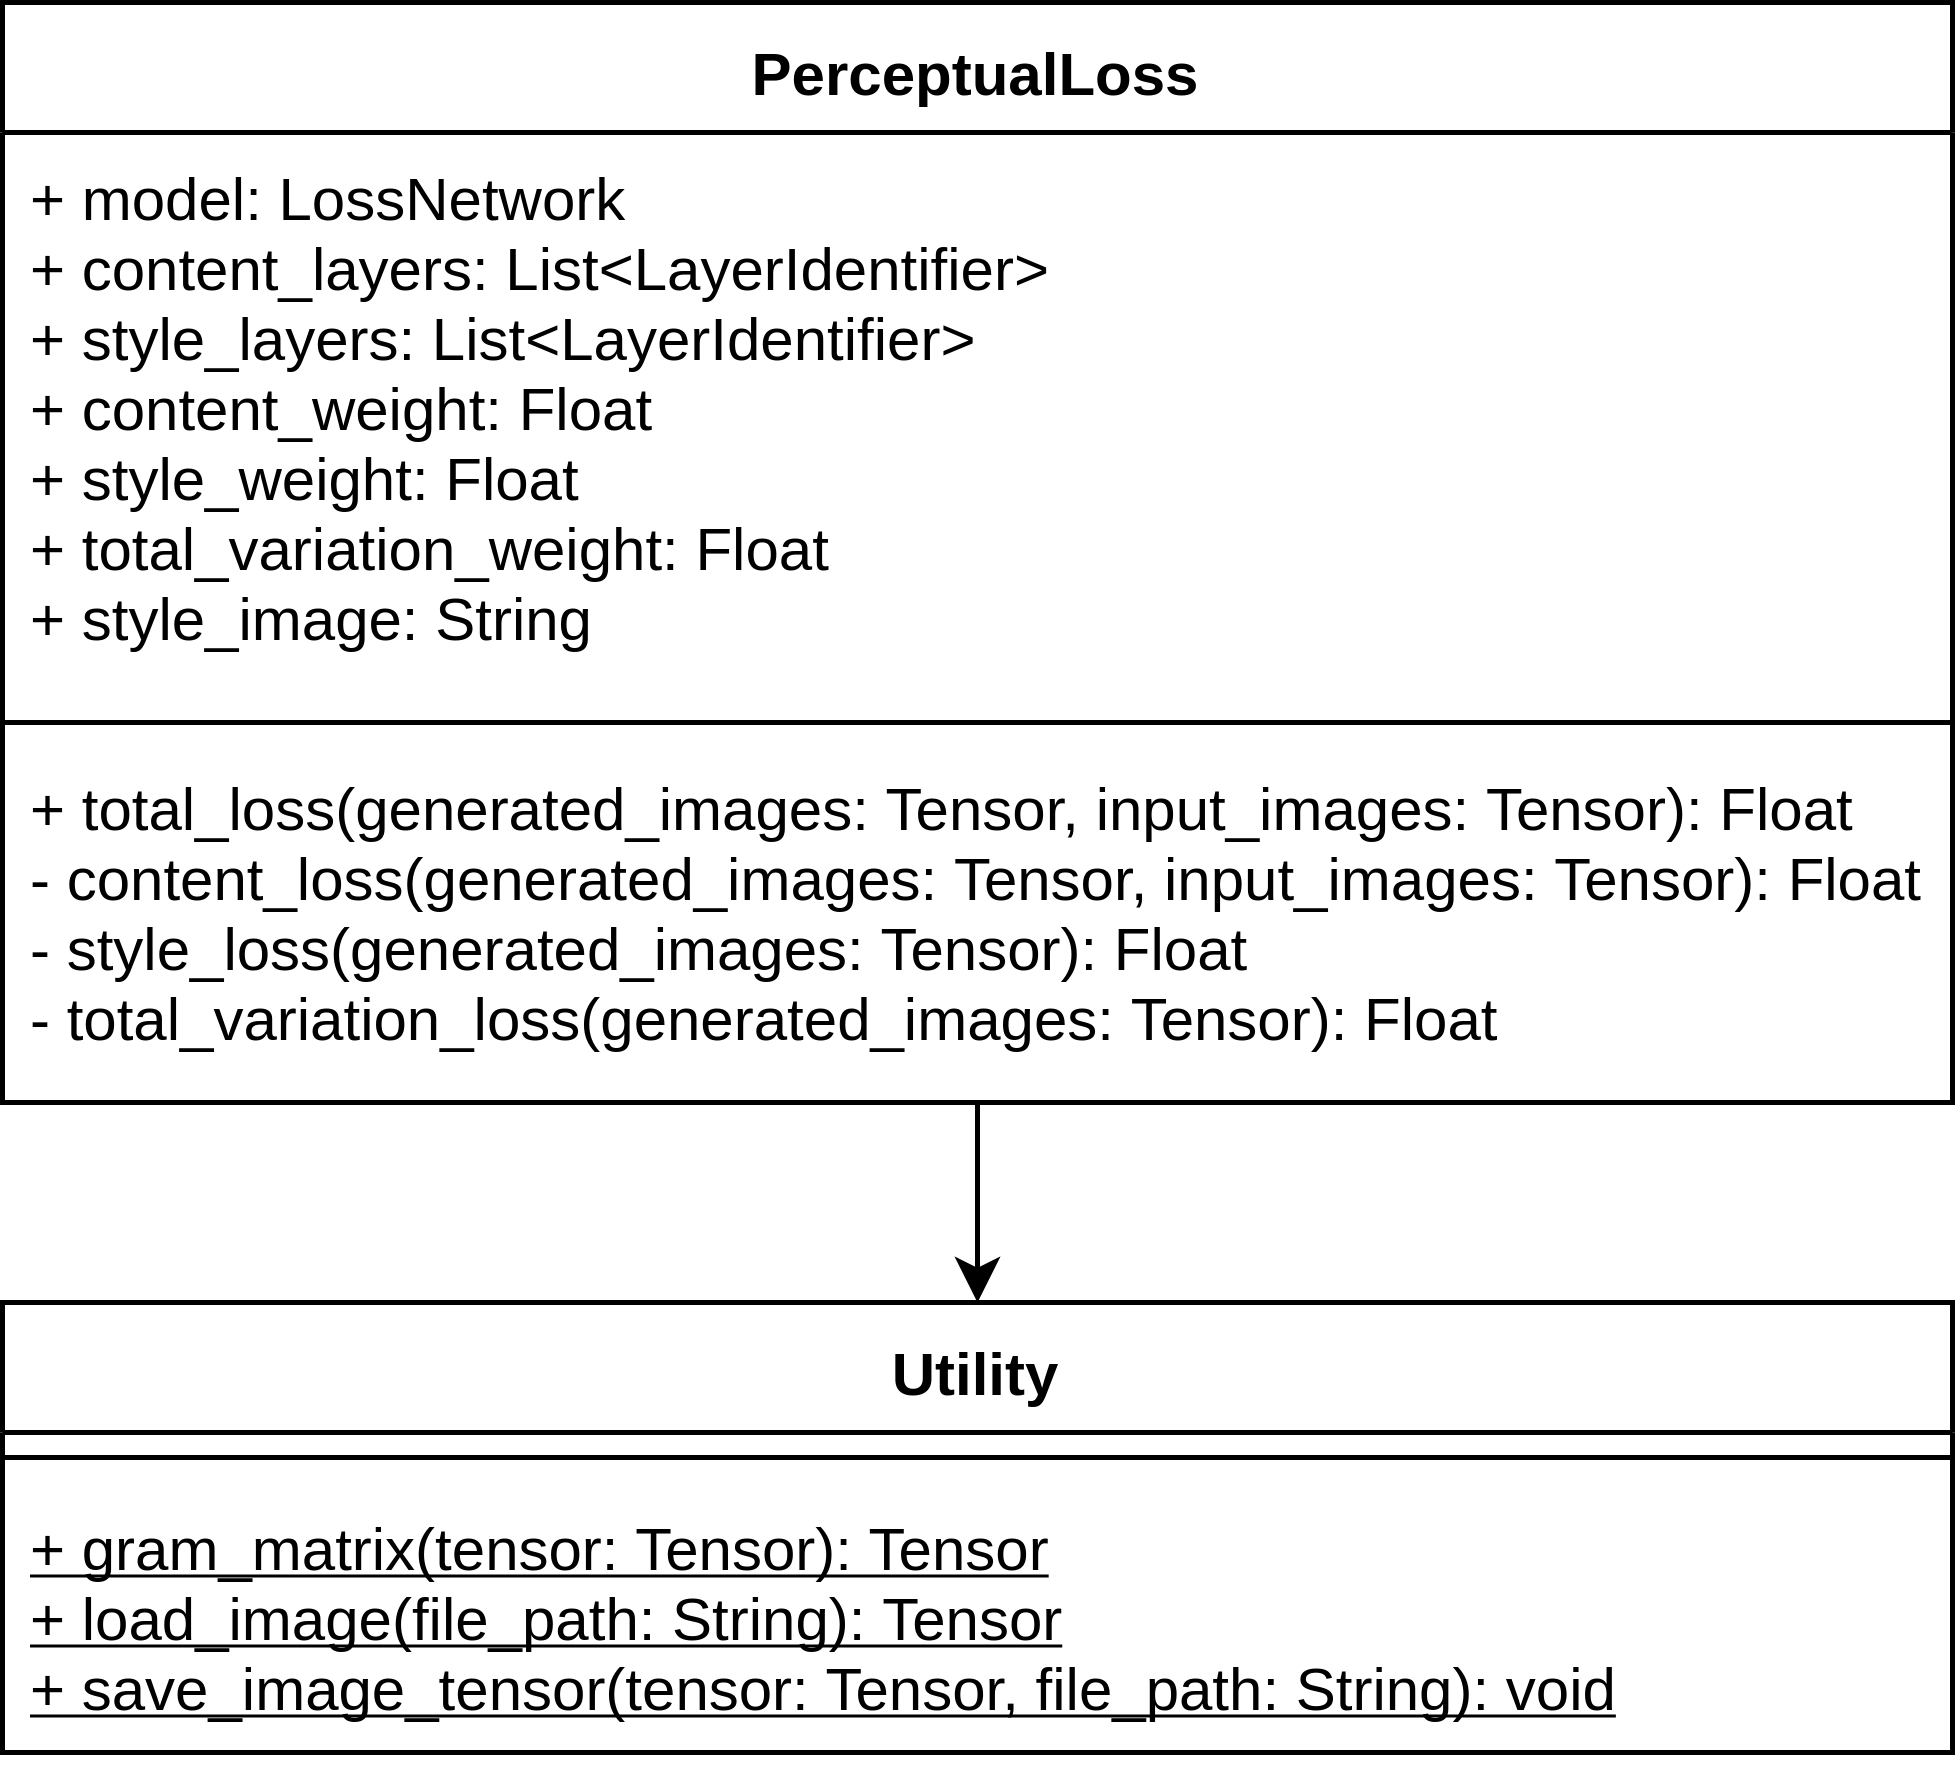
\includegraphics[width=0.50\textwidth]{resources/content/neural_style_class_diagram.png}
	\caption{Komponenten für den Neural Style Algorithmus, eigene Darstellung}
	\label{img:neural_style_class_diagram_img}
\end{figure}

Der Algorithmus wird in einer interaktiven Umgebung erstellt, damit unterschiedliche Kombinationen der Hyperparameter schnell verändert und getestet werden können. Folgender Programmablaufplan skizziert ein entsprechendes Script. Für die Berechnung der mathematisch aufwendigen Aufgaben (z.B. Backpropagation \ref{sec:backpropagation}) wird eine entsprechende externe Library, die für diesbezügliche Aufgaben optimiert wurde, benutzt.

% https://drive.google.com/file/d/1OVpNUtWEs0HbToxkkzMw6EZe5UUVHyme/view?usp=sharing
\begin{figure}[H]
	\centering
	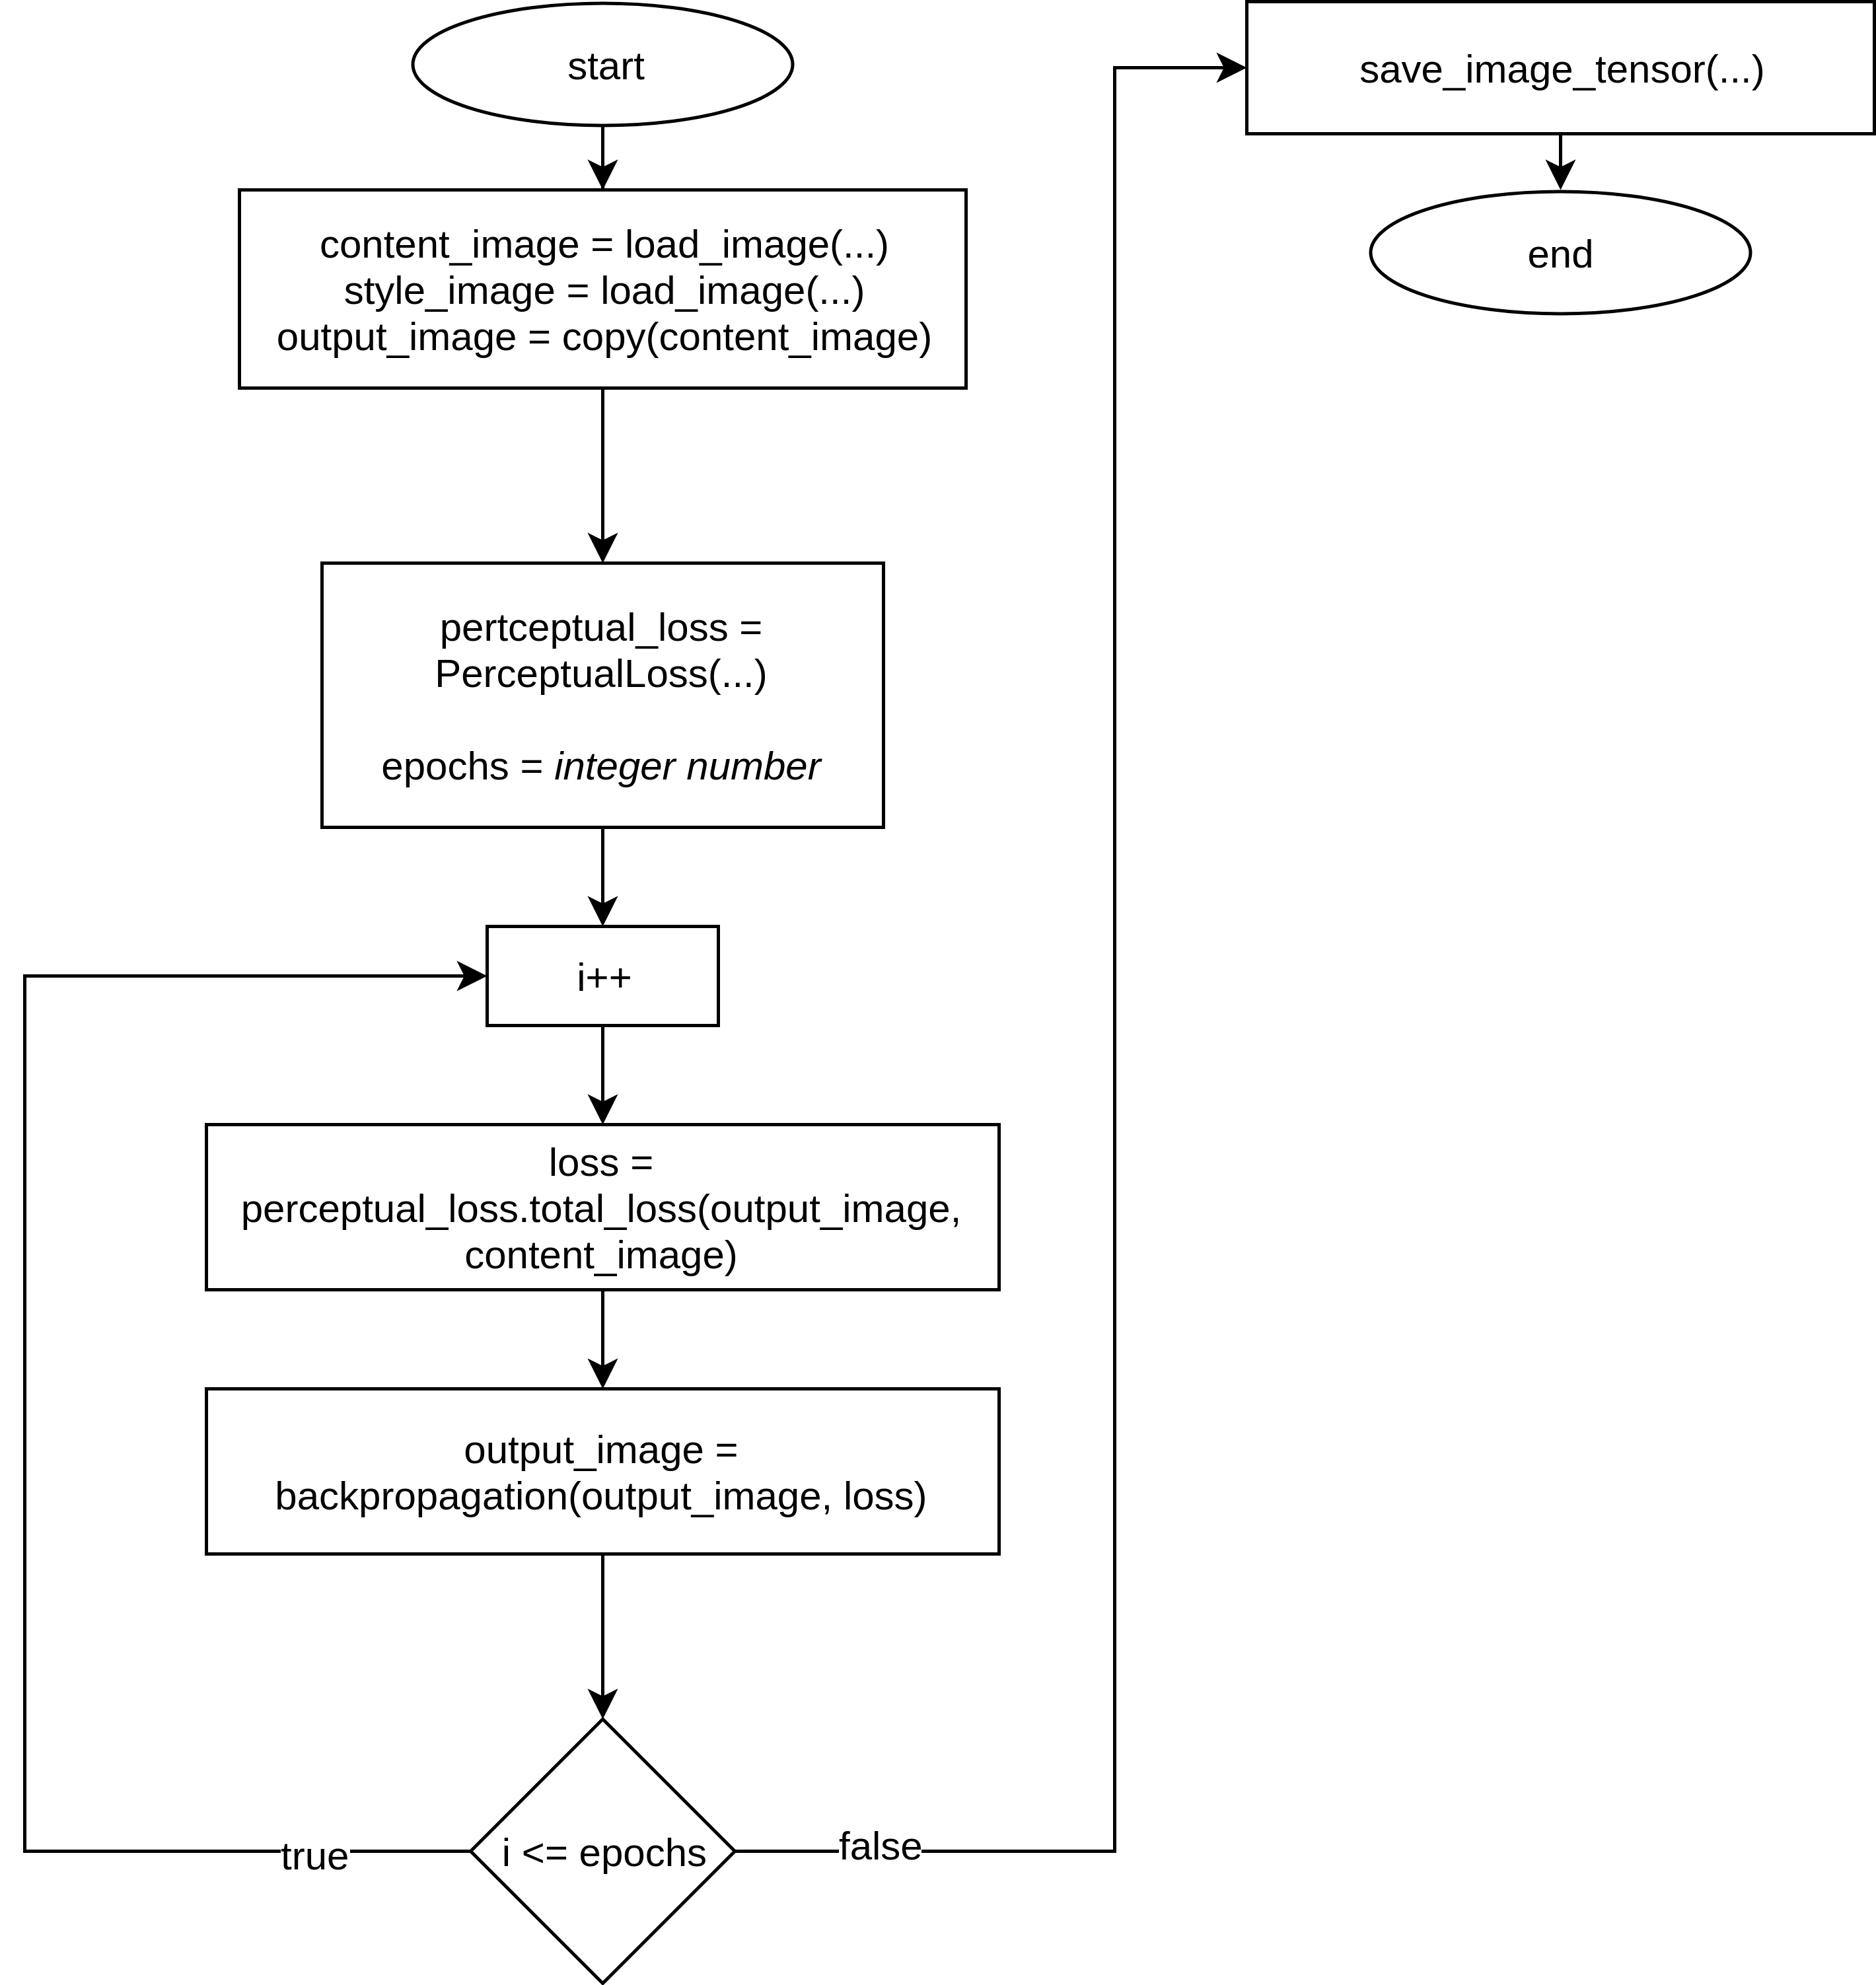
\includegraphics[width=1.0\textwidth]{resources/content/neural_style_pap.png}
	\caption{Programmablaufplan für den Neural Style Algorithmus, eigene Darstellung}
	\label{img:neural_style_pap_img}
\end{figure}

Bei Start des Programms werden das Content-Bild \mintinline{python}{content_image} und das Style-Bild \mintinline{python}{style_image} geladen. Danach wird eine Kopie von \mintinline{python}{content_image} in \mintinline{python}{output_image} erstellt. Die Bilder liegen dann als \gls{tensor}en der Form $ Channel \times Height \times Width $ vor, wobei $ Channel = 3 $ beträgt, da Bilder im RGB-Farbraum drei Farbkanäle aufweisen.

Es wird ein Objekt der Klasse \mintinline{python}{PerceptualLoss} erstellt. Bei der Instanziierung werden die folgenden benötigten Hyperparameter als Argumente dem Konstruktor übergeben:

\begin{itemize}
	\item \mintinline{python}{model}: Das Netzwerk, hier VGG16, dessen \gls{activation_map}s genutzt werden.
	\item \mintinline{python}{content_layers}: Eine Liste von Layern für die Berechnung des Content-Loss.\\ $ \{ relu3\_3 \} $
	\item \mintinline{python}{style_layers}: Eine Liste von Layern für die Berechnung des Style-Loss.\\ $ \{ relu1\_2, relu2\_2, relu3\_3, relu4\_3 \} $
	\item \mintinline{python}{content_weight}: Die Gewichtung des Content-Loss. $ 1 $ 
	\item \mintinline{python}{style_weight}: Die Gewichtung des Style-Loss. $ 1 \times 10^{7} $
	\item \mintinline{python}{total_variation_weight}: Die Gewichtung des Total-Variation-Denoising Faktors. $ 1 \times 10^{-5} $
	\item \mintinline{python}{style_image}: Der \gls{tensor} des gewünschten Style-Bildes.
\end{itemize}

Die Werte orientieren sich an den im Paper \cite{DBLP:journals/corr/JohnsonAL16} verwendeten Hyperparametern. Je nach gewähltem Stil sind jedoch abweichende Einstellungen erforderlich, um optisch ansprechende Ergebnisse zu erzielen. Auf unterschiedliche Kombinationen der Hyperparameter wird im Kapitel \ref{cha:tests} eingegangen.

\section{Fast Neural Style Transfer}

Die zuvor konzipierte Loss-Funktion kann beim Fast Neural Style Transfer wieder verwendet werden. 
Im Gegensatz zum vorherigen Verfahren werden nicht die Pixel als Parameter anhand der Loss-Funktion optimiert, sondern die Gewichtungsparameter eines Neuronalen Netzwerks. Dieses Verfahren wird auch Training genannt. Nach beendeter Trainingsphase ist das Netzwerk in der Lage, willkürliche Bilder in Bilder mit dem mit \mintinline{python}{style_image} ausgewählten Stil umzuwandeln.

Im Zuge dieser Arbeit soll eine Netzwerkarchitektur gefunden werden, die in der Lage ist, diese Aufgabe zu bewältigen. Außerdem wird die Netzwerkarchitektur im Kapitel \ref{cha:tests} auf ihre Performanz auf Geräten mit leistungsarmer Hardware getestet.

\subsection{Aufbau}
\label{sec:aufbau}

Die Netzwerkarchitektur, die beim Fast Neural Style Transfer verwendet wird, nachfolgend Transformer Net genannt, orientiert sich an dem Github-Repository \cite{PyTorchFastNeuralStyle}, das den Fast Neural Style Transfer implementiert.
Sie besteht aus drei Teilen. Einem Down-Sampling-Teil, einem Computational-Teil (auch Bottleneck genannt) und einem Up-Sampling-Teil.

\begin{figure}[H]
	\centering
	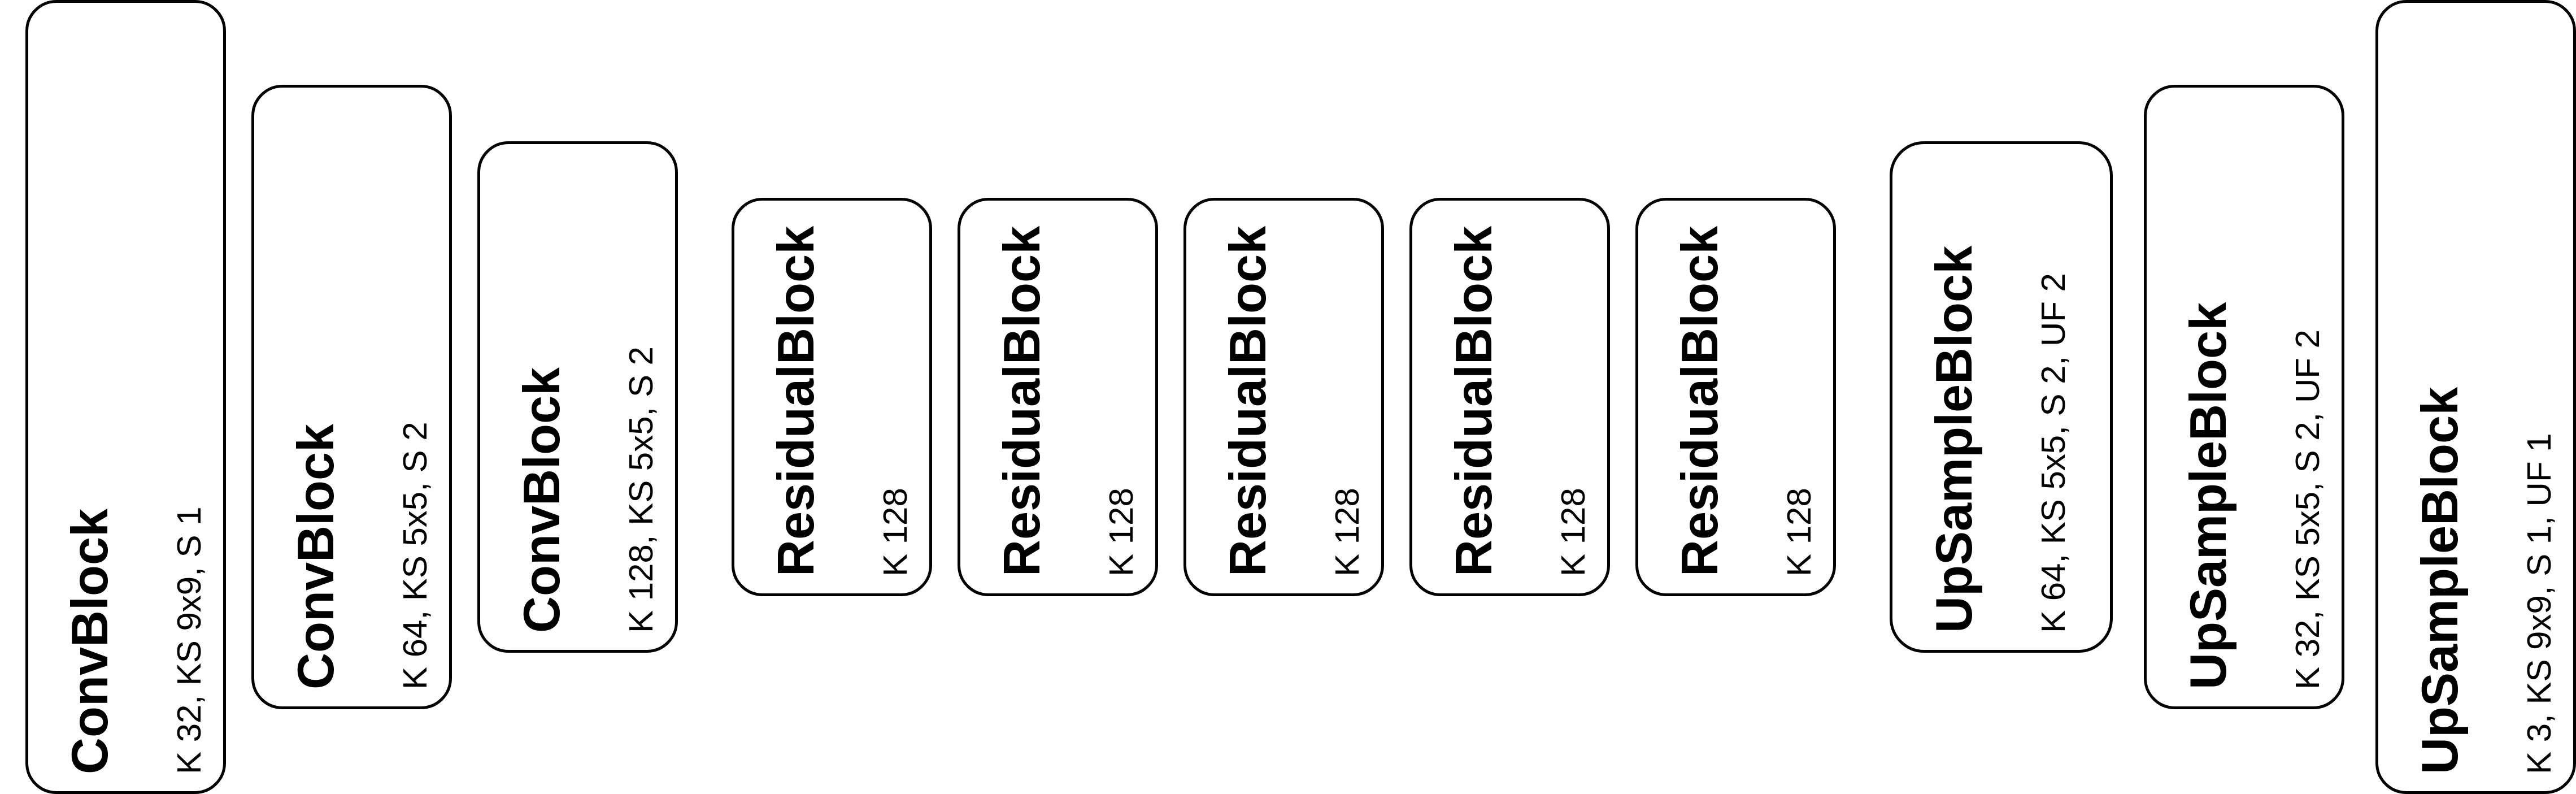
\includegraphics[width=1.0\textwidth]{resources/content/transformer_net.png}
	\caption{Netzwerkarchitektur des Transformer Net, eigene Darstellung}
	\label{img:transformer_net_img}
\end{figure}

Die Abkürzungen in der Grafik stehen für folgende Werte:

\begin{itemize}
	\item K = Anzahl Kernel
	\item KS = Kernel Size
	\item S = Stride
	\item UF = Upsampling Factor
\end{itemize}

Im ersten Teil, bestehend aus Convolutional Blöcken, wird durch die Verwendung des Stride Parameters das Eingangsbild hinter jedem Layer verkleinert. Mit einem Stride von 2 wird das Bild ungefähr auf die Hälfte der ursprünglichen Größe verkleinert, vgl. Kapitel \ref{cha:fundamentals}. Die Anzahl der Channels wird mit jedem Block vergrößert, um den Informationsverlust, der durch die verkleinerten Bilder entsteht, auszugleichen.

\begin{figure}[H]
	\centering
	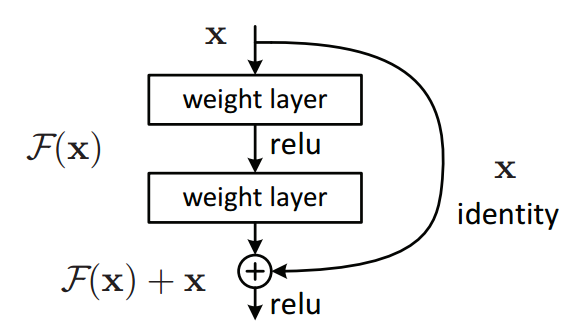
\includegraphics[width=0.50\textwidth]{resources/content/residual_block.png}
	\caption{Aufbau eines Residual Block \cite{residual_block_img}}
	\label{img:residual_block_img}
\end{figure}

Der zweite Teil besteht aus Residual Blöcken, beschrieben in \cite{DBLP:journals/corr/HeZRS15}. Diese bestehen aus zwei aufeinanderfolgenden Convolutional Layern, die mit einer sogenannten Skip-Connection mit ihren Eingangsdaten verbunden sind. Das hat den Vorteil, dass die ursprünglichen Eingangsdaten nach jedem Layer noch vorhanden sind. Dies beugt dem \gls{vanishing_gradient} Problem vor. In diesem Teil des Netzwerk entsteht die meiste Berechnung und die meisten Daten des Stils werden hier in den Gewichten der Kernels gespeichert.

Im dritten Teil wird das Bild durch Upsampling wieder auf seine ursprünglichen Maße vergrößert. Außerdem werden die Channels auf drei reduziert, um es als RGB-Bild anzeigen zu können. Die Vergrößerung wird durch Nearest Neighbor Interpolation kombiniert mit einem Convolutional Layer realisiert. Es wird zusammen mit seinen Vorteilen in \cite{odena2016deconvolution} näher beschrieben.

\pagebreak

\subsection{Unterschiedliche Netzwerkgrößen}

Wie auf der Grafik \ref{img:transformer_net_img} zu erkennen, ergibt sich die Anzahl der Channels jeweils aus einem Potenzwert der Basis $ 2 $ multipliziert mit einem Multiplikator $ m $, in diesem Fall der Wert $ 32 $.

\begin{align}
	& c_{1}(m) = m * 2^{0}
	& 32 = 32 * x^{0}
\end{align}

\begin{align}
	& c_{2}(m) = m * 2^{1}
	& 64 = 32 * x^{1}
\end{align}

\begin{align}
	& c_{3}(m) = m * 2^{2}
	& 128 = 32 * x^{2}
\end{align}

Durch den Multiplikator $ m $ lässt sich Netzwerkgröße und somit die Anzahl der Parameter einstellen. Unterschiedliche Netzwerkgrößen sind in der Lage, die Stile unterschiedlich gut festzuhalten. Auch wirkt sich die Netzwerkgröße auf die Berechnungs- und Trainingszeit des Netzwerks aus, was unter dem Gesichtspunkt der Verwendung auf Geräten mit leistungsarmer Hardware eine Rolle spielt.

Neben dem Multiplikator gibt es einen weiteren Parameter, der die Netzwerkgröße verändert. Der Parameter $ s $ legt die Anzahl der ResidualBlocks im Computational-Teil fest. Im Kapitel \ref{cha:tests} werden unterschiedliche Netzwerkgrößen und ihre Performanz getestet. \clearpage
\chapter{Implementierung}
\label{cha:implementation}

Im Bereich des Machine Learning und Deep Learning gibt es viele verschiedene Frameworks, die bei der Umsetzung und dem Training von Neuronalen Netzwerken behilflich sind. Beispiele hierfür sind Tensorflow\footnote{\url{https://www.tensorflow.org/}} von Google, PyTorch\footnote{\url{https://pytorch.org/}} von Facebook und Apache MXNet\footnote{\url{https://mxnet.apache.org/}}. Da bereits im Vorfeld dieser Arbeit Erfahrungen mit PyTorch gesammelt wurden, wurde diese Framework ausgesucht.

\section{Loss-Funktion}

Im ersten Schritt wird die Loss-Funktion implementiert, die das Kernstück des modellbasierten und des optimierenden Ansatzes ist.
PyTorch beinhaltet bereits vortrainierte Versionen verschiedener Modellarchitekturen. In dieser Arbeit wird das \gls{vgg16}-Modell benutzt, auf dieses wird mit \mintinline{python}{model = torchvision.models.vgg16(pretrained=True).features} zugegriffen. Das PyTorch-Modell ist dabei in die Bereiche \textit{features} und \textit{classifier} aufgeteilt. Es wird lediglich der Bereich \textit{features} benötigt, welcher die bereits vortrainierten Convolutional-Layer enthält. Der Bereich \textit{classifier} enthält die Fully-Connected-Layer des Modells, welche für die Aufgabenstellen ungenutzt bleiben.

\pagebreak

\subsection{Zugriff auf Hidden-Layer-Ergebnisse}

Um bei PyTorch auf Zwischenergebnisse der Hidden-Layer zuzugreifen, werden hinter diesen Hooks implementiert. Das kann in eine Funktion ausgelagert werden, welche die \gls{activation_map}s während der Berechnung des Forward-Pass durch das \gls{vgg16}-Modell extrahiert.

\begin{listing}[H]
\begin{minted}{python}
def extract_activation_maps(image_batch, model, layers, detach=False):
    class SaveActivationMap:
        def __init__(self):
            self.activation = []
        def hook(self, model, inpt, outpt):
            self.activation.append(outpt.detach() if detach else outpt)

    sam = SaveActivationMap()
    handles = []

    for layer in layers:
        i = list(dict(model.named_children()).keys()).index(str(layer))
        handles.append(model[i].register_forward_hook(sam.hook))
    model(image_batch)

    for handle in handles:
        handle.remove()

    return sam.activation
\end{minted}
\captionof{lstlisting}{Extrahierung der Activation-Maps mit PyTorch}
\end{listing}

\subsection{Content-Loss}

Um das Content-Loss zu bilden, wird mit der zuvor definierten Funktion auf die Zwischenergebnisse der Hidden-Layer zugegriffen.
Das Ergebnis ist das \gls{mse_loss} aller Zwischenergebnisse der Eingangsdaten (Inhaltsbild) verglichen mit den Zwischenergebnissen der Ausgangsdaten (generierte Bilder), vgl. Kapitel \ref{sec:content_loss}.

\begin{listing}[H]
\begin{minted}{python}
def content_loss(self, y, x):
    y = extract_activation_maps(y, self.model, self.c_layers)
    x = extract_activation_maps(x, self.model, self.c_layers, detach=True)
    return sum([
        F.mse_loss(generated_feature, input_feature)
        for generated_feature, input_feature in zip(y, x)
    ])
\end{minted}
\captionof{lstlisting}{Berechnung des Content-Loss, vgl. Gleichung \eqref{eq:content_loss}}
\end{listing}

\subsection{Style-Loss}

Für das Style-Loss wird eine Funktion benötigt, um die Gram-Matrix eines \gls{tensor}s zu bilden. Die Anzahl der Dimensionen des Eingangstensors wird auf zwei Dimensionen geflächt. Diese Matrix wird mit einer von sich selbst transponierten Version multipliziert. Danach wird das Ergebnis über das Produkt der Anzahl der Channel, Höhe und Breite des Eingangstensors normalisiert.

\begin{listing}[H]
\begin{minted}{python}
def gram_matrix(tensor):
    b, c, h, w = tensor.shape
    normalizer = c * h * w
    tensor_flat = tensor.flatten(2)

    return torch.div(
        torch.bmm(tensor_flat, tensor_flat.transpose(1, 2)),
        normalizer
    )
\end{minted}
\captionof{lstlisting}{Berechnung der Gram-Matrix, vgl. Gleichungen \eqref{eq:gram_matrix_1} u. \eqref{eq:gram_matrix_2}}
\end{listing}

Die Gram-Matrix-Funktion wird dazu benutzt, das Style-Loss zu berechnen. Wie beim Content-Loss wird das \gls{mse_loss} gebildet. Dazu werden vorher die Gram-Matrizen aller \gls{activation_map}s berechnet. Auf diese Weise wird das berechnete Ausgangsbild mit dem vorher eingestellten Stilbild verglichen. In dieser Implementierung wurde die Gewichtung der einzelnen Layer nicht berücksichtigt. Die Implementierung weicht daher geringfügig von der in den Grundlagen verwendeten Gleichung \eqref{eq:style_loss} ab.

\begin{listing}[H]
\begin{minted}{python}
def style_loss(self, y):
    y = extract_activation_maps(y, self.model, self.s_layers)
    y_grams = [gram_matrix(row) for row in y]

    return sum([
        F.mse_loss(y_gram, style_gram)
        for y_gram, style_gram in zip(y_grams, self.style_grams)
    ])
\end{minted}
\captionof{lstlisting}{Berechnung des Style-Loss, vgl. Gleichung \eqref{eq:style_loss}}
\end{listing}

\pagebreak

\subsection{Total-Variation-Loss}

Das Total-Variation-Loss berechnet die Summe der Abweichungen eines Pixels zum nächsten Pixel eines Bildes. Dies wird für Höhe und Breite des Bildes durchgeführt und addiert.

\begin{listing}[H]
\begin{minted}{python}
def total_variation_loss(self, y):
    return torch.add(
        torch.sum(torch.abs(y[:, :, :, :-1] - y[:, :, :, 1:])),
        torch.sum(torch.abs(y[:, :, :-1, :] - y[:, :, 1:, :]))
    )
\end{minted}
\captionof{lstlisting}{Berechnung des Total-Variation-Loss \cite{pytorch-implementation-of-perceptual-losses-for-real-time-style-transfer}, vgl. Gleichung \eqref{eq:total_variation_loss}}
\end{listing}

\subsection{Perceptual-Loss}

Das Perceptual-Loss ist das Gesamt-Loss und addiert die einzelnen Teil-Losse mit entsprechend einstellbaren Gewichtungsfaktoren.

\begin{listing}[H]
\begin{minted}{python}
def forward(self, y, x):
    content_loss = self.c_weight * self.content_loss(y, x)
    style_loss = self.s_weight * self.style_loss(y)
    total_variation_loss = self.tv_weight * self.total_variation_loss(y)

    loss = content_loss + style_loss + total_variation_loss

    return loss
\end{minted}
\captionof{lstlisting}{Berechnung des gesamten Perceptual-Loss, vgl. Gleichung \eqref{eq:perceptual_loss}}
\end{listing}

\section{Neural Style Transfer}

Die Implementierung des Neural Style Transfer Algorithmus wird in einem Jupyter Notebook\footnote{\url{https://jupyter.org/}} durchgeführt. 
Dadurch können im späteren Verlauf unterschiedliche Tests durchgeführt werden, da die Hyperparameter schnell angepasst werden können.

Das Notebook, vgl. \ref{sec:nootebook_neural_style_transfer}, orientiert sich am zuvor erstellten Programmablaufplan, vlg. Abbildung \ref{img:neural_style_pap_img}. Es bietet außerdem die Auswahl zwischen den PyTorch-Optimizern \gls{adam} und L-BFGS \cite{Liu1989}. Folgender Code zeigt die Optimierung von Parametern mit PyTorch.

\begin{listing}[H]
\begin{minted}{python}
criterion = PerceptualLoss(...)
optimizer = optim.Adam([outputs])

for epoch in range(epochs):
    optimizer.zero_grad()

    loss = criterion(outputs, inputs)
    loss.backward()

    optimizer.step()    
\end{minted}
\captionof{lstlisting}{Vereinfachter Code einer Trainingsschleife in PyTorch}
\end{listing}

\section{Fast Neural Style Transfer}

Das Verfahren des Fast Neural Style funktioniert ähnlich wie beim vorher vorgestellten Neural Style Transfer. Anstatt der Pixel des Ausgangsbildes werden jedoch die Gewichte eines Neuronalen Netzwerks optimiert. Der bestehende Code kann aus  dem vorherigen Kapitel wiederverwendet werden. Lediglich die Initialisierung des PyTorch Optimizers muss angepasst werden.

\begin{listing}[H]
\begin{minted}{python}
model = TransformerNet(...)
optimizer = optim.Adam(model.parameters())
\end{minted}
\captionof{lstlisting}{Optimierung der Gewichte des Netzwerk}
\end{listing}

\subsection{COCO-Datensatz}

Um das Neuronale Netzwerk zu trainieren, wird ein großer Bilddatensatz benötigt. In dieser Arbeit wird dafür der \gls{coco}-Datensatz der Firma Microsoft verwendet \cite{DBLP:journals/corr/LinMBHPRDZ14}. Es handelt sich dabei um einen öffentlichen, frei verfügbaren Datensatz vieler verschiedener Bilder unterschiedlicher Kategorien. Während des Trainingsverlaufs werden zufällige Bilder aus dem \gls{coco}-Datensatz genutzt und das Loss  (Style-, Content- und Total-Variation-Loss) über die Ausgaben, die das Netzwerk generiert, berechnet. Mit dem berechneten Loss ist PyTorch in der Lage, die Gradienten der Gewichte des Neuronalen Netzwerks zu berechnen und diese schrittweise zu optimieren.

Der \gls{coco}-Datensatz liegt in Form vieler verschiedener \gls{jpeg}-Bilder vor. Um nicht alle Bilder gleichzeitig laden zu müssen, bietet PyTorch die Möglichkeit, einen Dataloader\footnote{Weitere Information zum PyTorch-Dataloader: \url{https://pytorch.org/tutorials/beginner/data_loading_tutorial.html}} zu nutzen, der die Bilder in der gewünschten Batchgröße Schritt für Schritt lädt.

\begin{listing}[H]
\begin{minted}{python}
dataset = datasets.ImageFolder(
    config['dataset_path'],
    transform=transforms.Compose([
        transforms.Resize(config['content_image_size']),
        transforms.CenterCrop(config['content_image_size']),
        transforms.ToTensor()
    ])
)

dataloader = data.DataLoader(dataset, batch_size=config['batch_size'], shuffle=True)
\end{minted}
\captionof{lstlisting}{Der PyTorch-Dataloader lädt Bilder in der gewünschten Batchgröße}
\end{listing}

Der Dataloader lädt alle Bilder in allen Unterordnern innerhalb des konfigurierten Pfades.

\subsection{Netzwerkarchitektur}
\label{sec:network_architecture}

Die Architektur des Neuronalen Netzes spielt eine wichtige Rolle. Sie muss in der Lage sein, die Eigenschaften eines Stils möglichst gut zu erlernen und dabei performant bleiben. Dabei wurde die in Kapitel \ref{sec:fast_neural_style_transfer} vorgestellte Netzwerkarchitektur des Image Transformer Networks implementiert. Dies geschieht in PyTorch in Form einer Klasse, welche von \mintinline{python}{Module} erbt.

Um in Kapitel \ref{cha:tests} das Testen unterschiedlicher Netzwerkarchitekturen zu ermöglichen, wird die Klasse des Image Transformer Networks möglichst dynamisch implementiert. Einstellbar sind dabei folgende Parameter, die im weiteren Verlauf erklärt werden:

\begin{itemize}
    \item channel\_multiplier
    \item bottleneck\_size
    \item bottleneck\_type
    \item final\_activation\_fn
    \item intermediate\_activation\_fn
\end{itemize}

\subsection{Aktivierungsfunktionen}

Für den dynamischen Aufbau des Netzwerks wird eine Funktion benötigt, die entsprechende PyTorch-Aktivierungsfunktionen zurückgibt. Hardtanh und Sigmoid kommen als finale Aktivierungsfunktionen des Netzwerks in Betracht, da Sie Werte zwischen $ 0.0 $ und $ 1.0 $ zurückliefern. Das eignet sich für die Generierung von Bildern, welche in PyTorch ebenfalls Pixelwerte zwischen $ 0.0 $ und $ 1.0 $ besitzen. Zu beachten ist, dass die Hardtanh-Funktion mit den Parametern \mintinline{python}{min_val=0.0} und \mintinline{python}{max_val=1.0} initialisiert wird, die den Wertebereich verschieben. Mit den Standardeinstellungen liegt der Wertebereich der Hardtanh-Funktion zwischen $ -1.0 $ und $ 1.0 $. Die Parameter \mintinline{python}{final_activation_fn} und \mintinline{python}{intermediate_activation_fn} werden dabei auf die entsprechenden PyTorch-Aktivierungsfunktionen überführt.

\subsection{ConvBlock}

Des weiteren müssen die in Kapitel \ref{sec:aufbau} konzipierten Layer-Blöcke implementiert werden. Der ConvBlock besteht aus den PyTorch-Layern \mintinline{python}{Conv2d}, \mintinline{python}{InstanceNorm2d} und der gewählten Aktivierungsfunktion. \mintinline{python}{InstanceNorm2d} wurde aufgrund des Papers \cite{DBLP:journals/corr/UlyanovVL16} gewählt und dort näher in Bezug auf die Verwendung mit Style Transfer-Methoden erläutert.

Die Parameter \mintinline{python}{in_channels} und \mintinline{python}{out_channels} ergeben sich aus dem Parameter \mintinline{python}{channel_multiplier} ($ m $) multipliziert mit einem festen Wert, der je nach Layer die Werte $ 1 $, $ 2 $ oder $ 4 $ beträgt.

\subsection{ResidualBlock}

Der ResidualBlock, vgl. \ref{img:residual_block_img}, besteht aus zwei aufeinanderfolgenden \mintinline{python}{Conv2d}-Layern. Wie beim vorherigen ConvBlock werden die Daten über \mintinline{python}{InstanceNorm2d} normalisiert, anschließend wird die Aktivierungsfunktion angewendet. Die Besonderheit ist, dass die Eingangsdaten kopiert und danach mit den berechneten Daten der Convolutional-Layer addiert werden. Durch \mintinline{python}{Conv2d} verkleinert sich die Dimension der Daten, vgl. \ref{sec:conv_networks}, was durch den \mintinline{python}{ReflectionPad2d}-Layer wieder ausgeglichen wird. Eingangsdaten und berechnete Daten müssen die gleichen Dimensionen aufweisen, um addiert werden zu können. Die Parameter \mintinline{python}{in_channels} und \mintinline{python}{out_channels} ergeben sich aus \mintinline{python}{channel_multiplier} multipliziert mit $ 4 $.

\subsection{UpSampleBlock}

Der UpSampleBlock schaltet lediglich dem ConvBlock ein Upsampling-Verfahren vor, um das Bild um einen entsprechenden Faktor zu vergrößern. In dieser Arbeit wird Nearest Neighbor Interpolation verwendet.

\subsection{TransformerNet}

Neben den Layer-Blöcken wurde noch die eigentliche Netzwerkarchitektur implementiert. Die Implementierung nimmt die in \ref{sec:network_architecture} beschriebenen Parameter im Konstruktor entgegen, um eine entsprechende Netzwerkarchitektur zu generieren. Neben den bereits beschriebenen Einstellungen gibt \mintinline{python}{bottleneck_size} die Anzahl der hintereinander geschalteten ResidualBlocks an. Der \mintinline{python}{bottleneck_type} ist für zukünftige Erweiterungen vorgesehen, damit der ResidualBlock durch einen anders aufgebauten Block ersetzt werden kann. Außerdem wurde ein anfängliches Padding eingefügt, um die ursprüngliche Bildgröße beizubehalten.

\subsection{Weitere Implementierungen}

Zusätzlich zu den bereits vorgestellten Implementierungen wurden Hilfsskripte und Jupyter Notebooks zum Testen erstellt. Außerdem wurde eine Trainer-Klasse entworfen, die in der Lage ist, Einstellungen für Trainingsläufe aus einer Konfigurationsdatei zu lesen und somit 
ein aufeinanderfolgendes Training mehrerer Modelle zu ermöglichen. Auf diese Art kann man viele unterschiedliche Parametereinstellungen testen.

Zur Realisierung eines Prototyps wurde eine JSON-API mit dem Framework Flask\footnote{Flask: \url{http://flask.pocoo.org/}} erstellt. Die API stellt einen Endpunkt zur Verfügung, welche den Style Transfer mit einem gewünschten Modell durchführt. Sie wurde in einen Docker\footnote{Docker: \url{https://www.docker.com/}}-Container überführt, um das Hosting auf unterschiedlichen Geräten zu erleichtern.

Um die Ergebnisse zu visualisieren, wurde eine Frontend-Applikation mit dem Framework Angular\footnote{Angular: \url{https://angular.io/}} erstellt. Diese kann Bilder über die Webcam eines Handys oder eines Computers aufnehmen und sie an die Flask-API senden, die nachfolgend das aufgenommene Bild in einen vorher ausgewählten Stil überführt.

Skripte, Frontend-Applikationen und JSON-API sind nicht Bestandteil dieser Arbeit und befinden sich in einem prototypischen Zustand. Der komplette Code zu diesem Projekt ist unter \url{https://github.com/christophstach/style-transfer-project} öffentlich einsehbar. Der Code des Frontends unter \url{https://github.com/christophstach/style-transfer-frontend}. Ein gehosteter Prototyp zum Testen des Style Transfers ist unter \url{https://stylized.christophstach.me/} verfügbar. \clearpage
\chapter{Tests und Experimente}
\label{cha:tests}

Im Kapitel Tests und Experimente werden unterschiedliche Hyperparameter-Konfigurationen auf ihre Auswirkungen getestet. Außerdem wird mit unterschiedlichen Netzwerkarchitekturen die Performanz auf Geräten mit leistungsarmer Hardware gemessen.

\section{Auswirkungen der Hyperparameter}

Im Folgenden werden unterschiedliche Kombinationen der Gewichtungsparameter Content-Weight $ \alpha $, Style-Weight $ \beta $ und Total-Variation-Weight $ \gamma $ getestet. Dabei wird als Inhaltsbild  eine eigene Abbildung der HTW-Berlin benutzt. Als Stilbild wird das Kunstwerk The Starry Night des Künstlers Vincent Van Gogh und The Scream von Edvard Munch verwendet. Die generierten Bilder entsprechen einer Größe von 768 * 768 Pixel. Die restlichen Hyperparameter werden aus dem Kapitel Methodologie \ref{sec:method_neural_style_transfer} übernommen.

\pagebreak

\subsection{Experiment 1: Starry Night}

In diesem Experiment wird das Stilbild The Starry Night von Vincent Van Gogh verwendet.

\begin{figure}[H]
    \centering
    \begin{subfigure}[h]{0.20\textwidth}
        \centering
        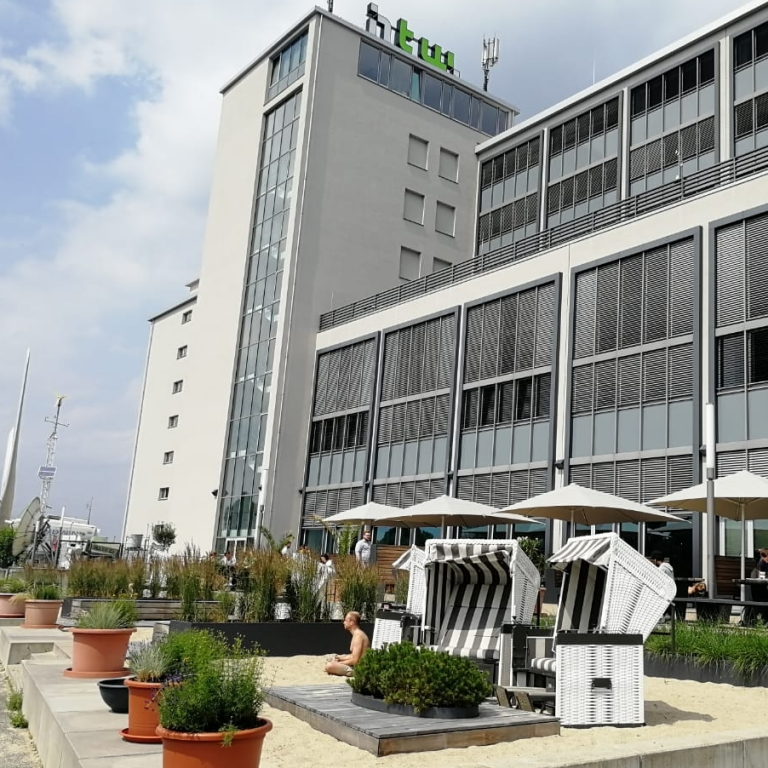
\includegraphics[width=\textwidth]{resources/content/content/htw-768x768.jpg}
    \end{subfigure}
    \begin{subfigure}[h]{0.20\textwidth}
        \centering
        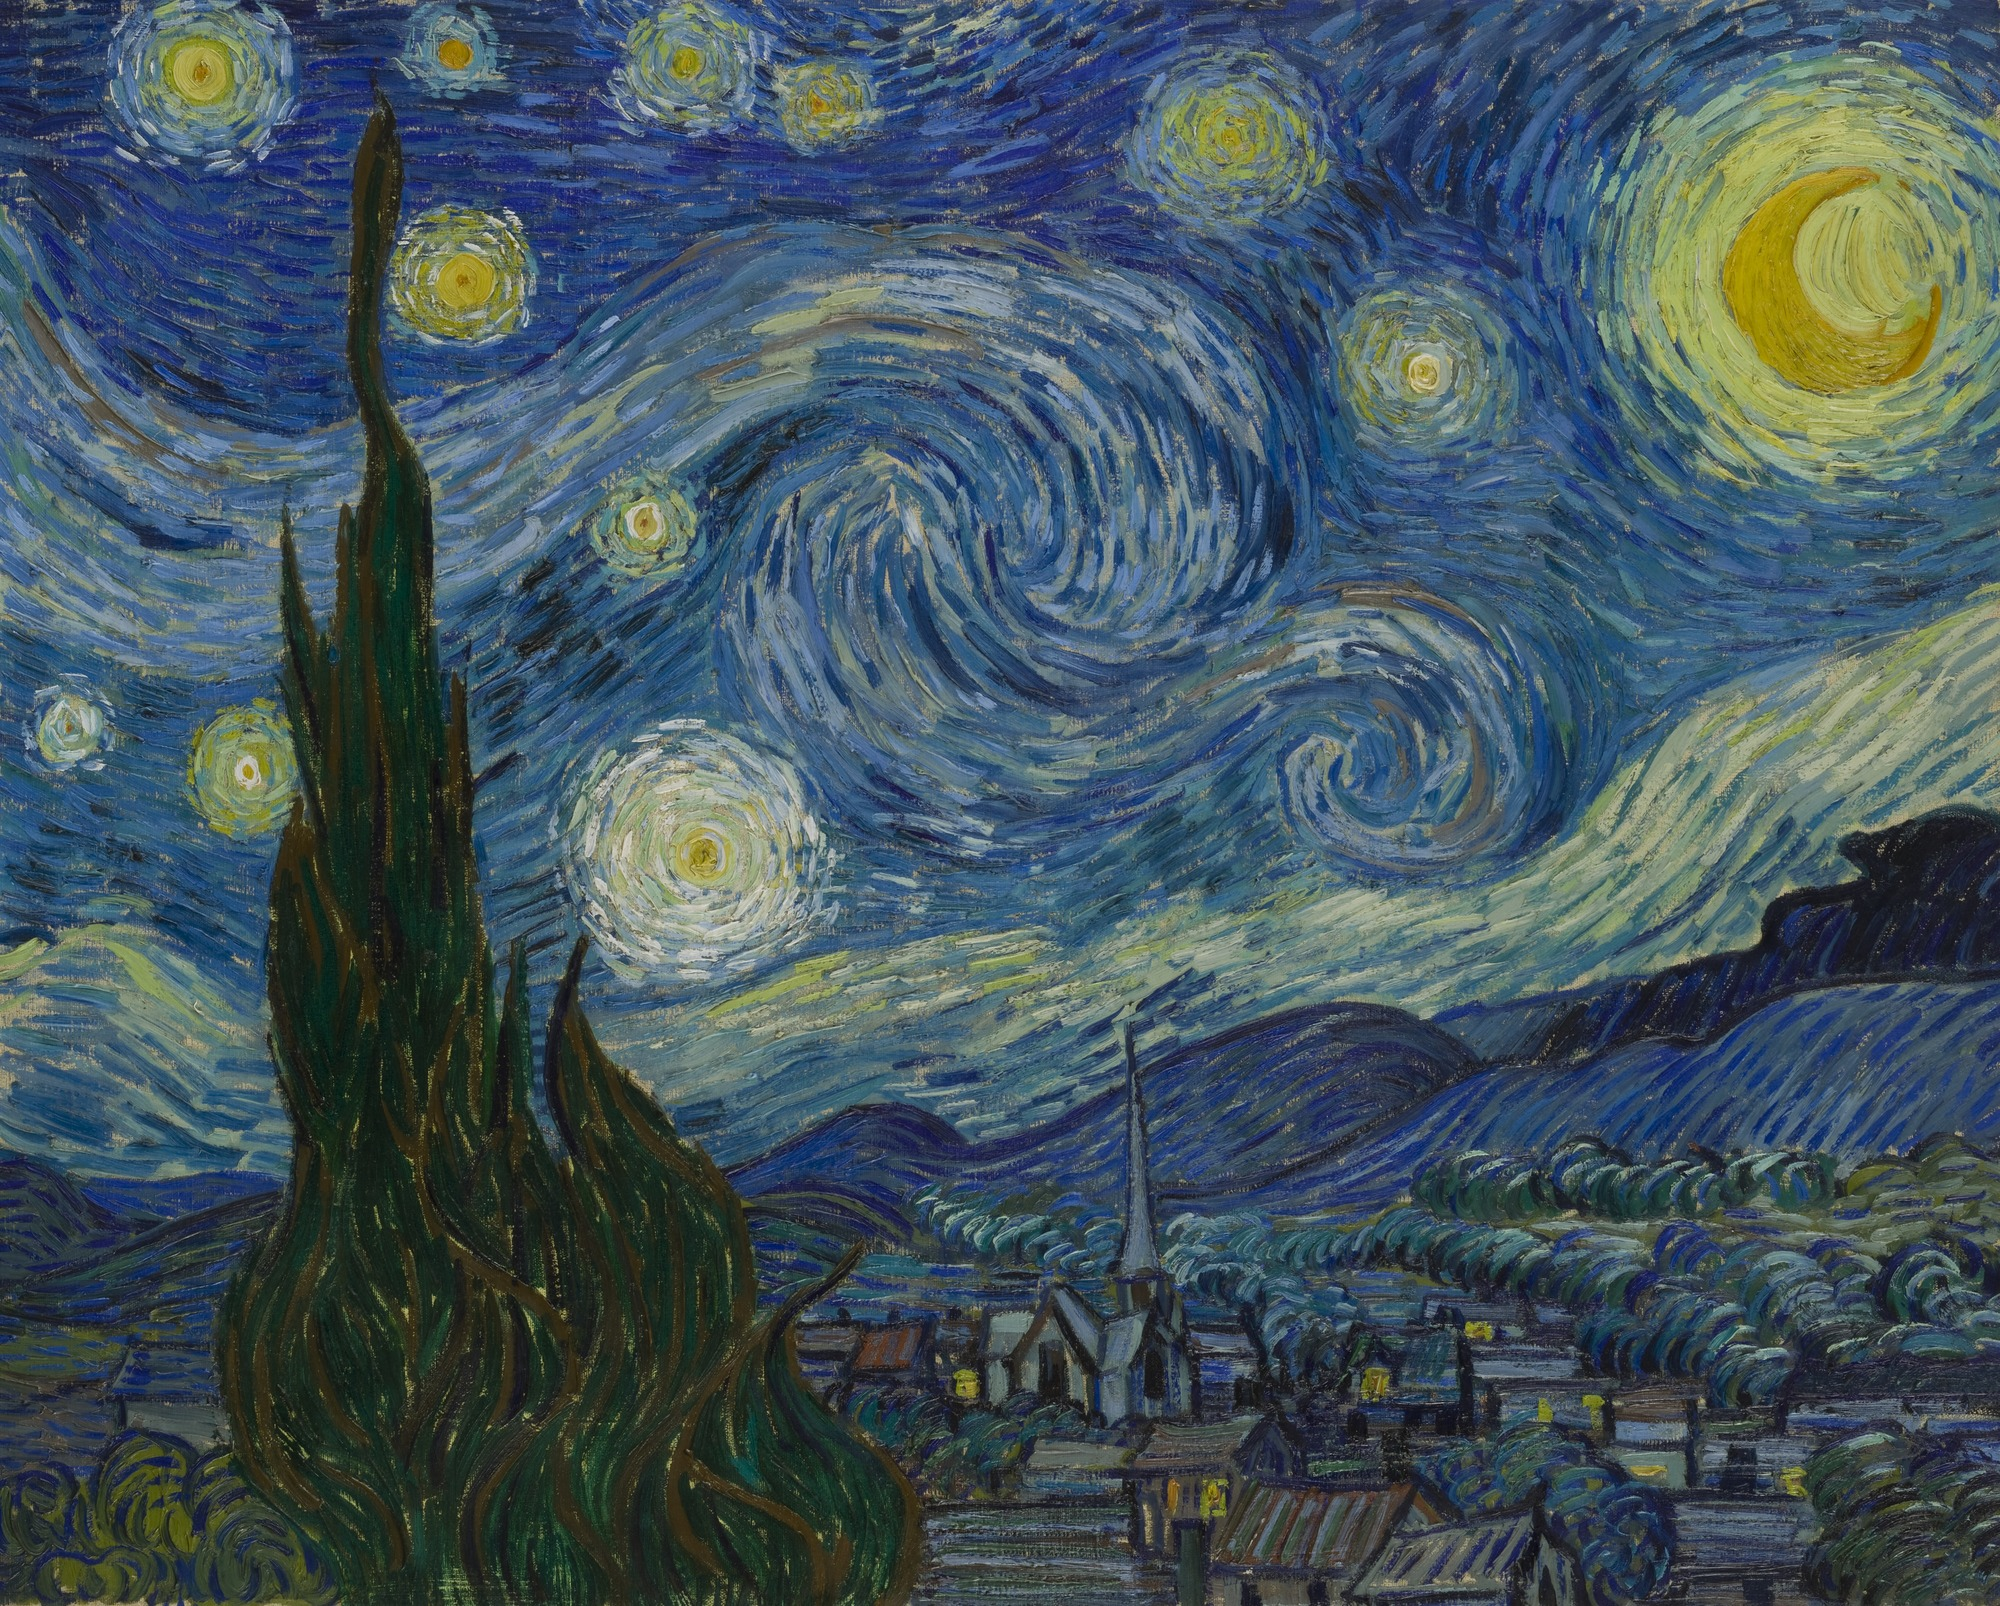
\includegraphics[width=\textwidth]{resources/content/style/starry_night.jpg}
    \end{subfigure}
    \caption{HTW kombiniert mit The Starry Night \cite{the_starry_night_img}}
\end{figure}

In der ersten Abbildungen werden die verschiedenen
Stilgewichtungen $ \beta = 10^{5} $, $ \beta = 10^{6} $, $ \beta = 10^{7} $, $ \beta = 10^{8} $ und $ \beta = 10^{9} $ für The Starry Night getestet.

\begin{figure}[H]
    \centering
    \begin{subfigure}[h]{0.15\textwidth}
        \centering
        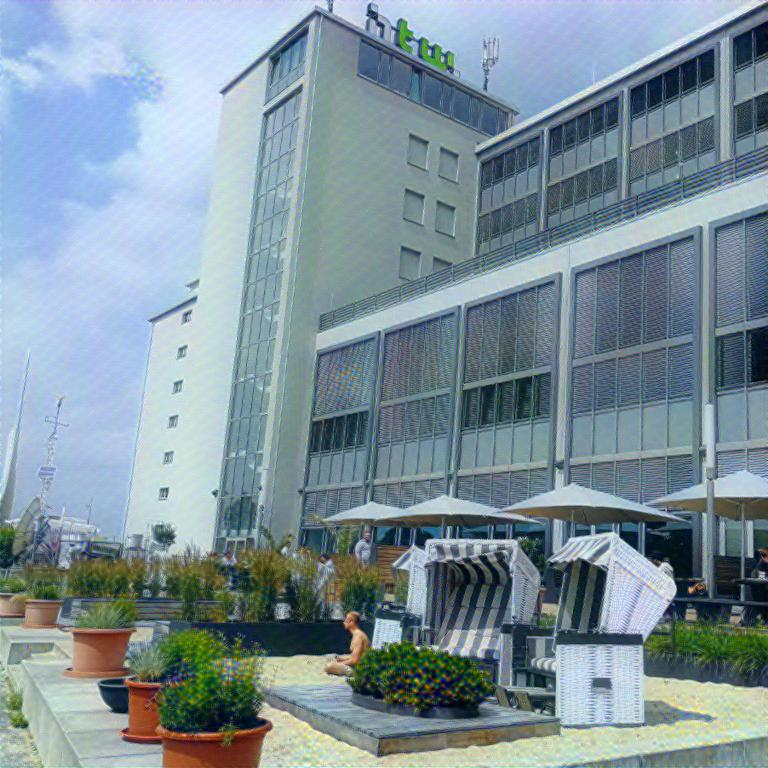
\includegraphics[width=\textwidth]{resources/content/experiments/a__starry_night__768x768__style-weight_1e+05__tv-weight_0e+00.jpg}
    \end{subfigure}
    \begin{subfigure}[h]{0.15\textwidth}
        \centering
        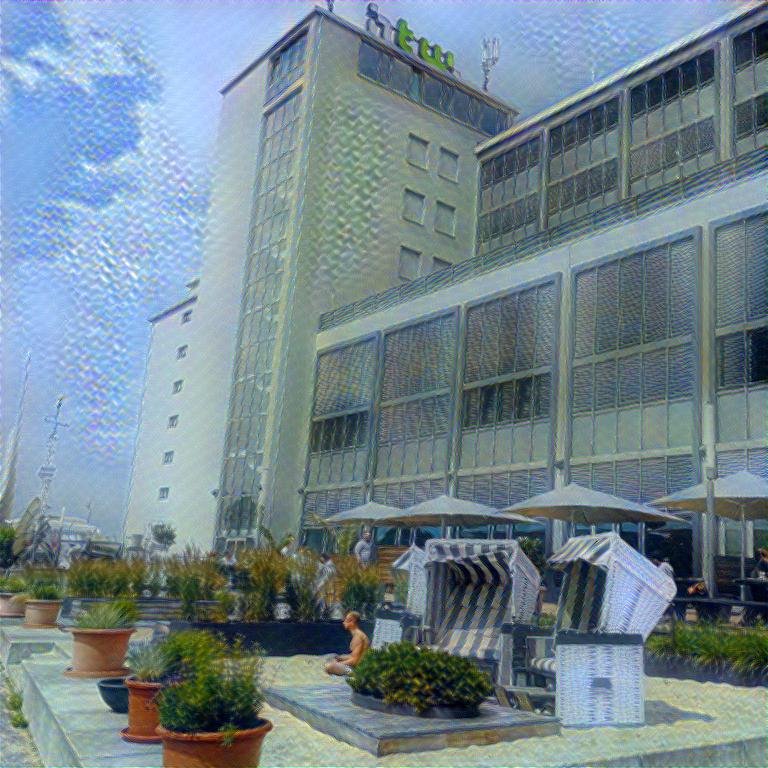
\includegraphics[width=\textwidth]{resources/content/experiments/a__starry_night__768x768__style-weight_1e+06__tv-weight_0e+00.jpg}
    \end{subfigure}
    \begin{subfigure}[h]{0.15\textwidth}
        \centering
        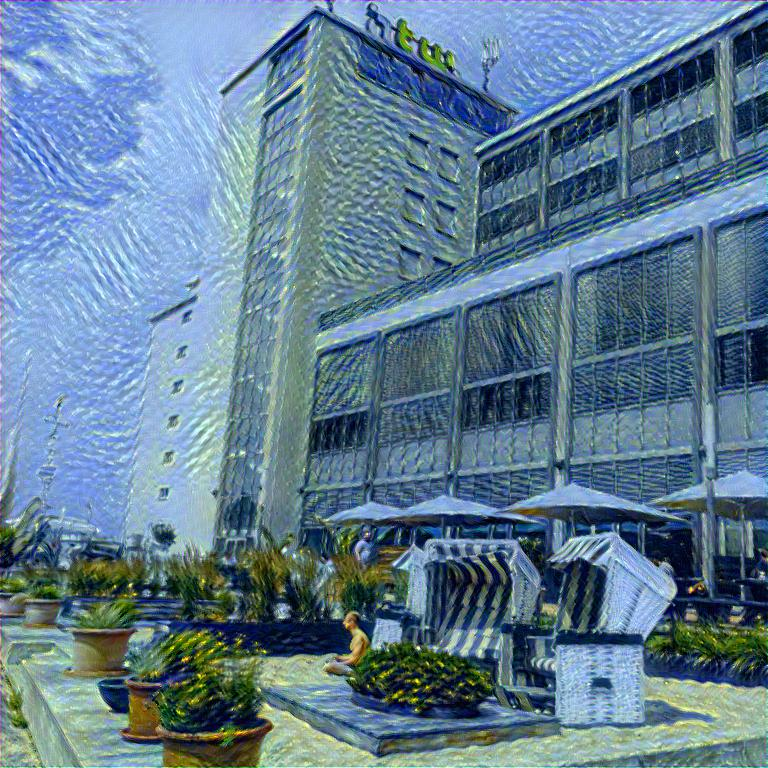
\includegraphics[width=\textwidth]{resources/content/experiments/a__starry_night__768x768__style-weight_1e+07__tv-weight_0e+00.jpg}
    \end{subfigure}
    \begin{subfigure}[h]{0.15\textwidth}
        \centering
        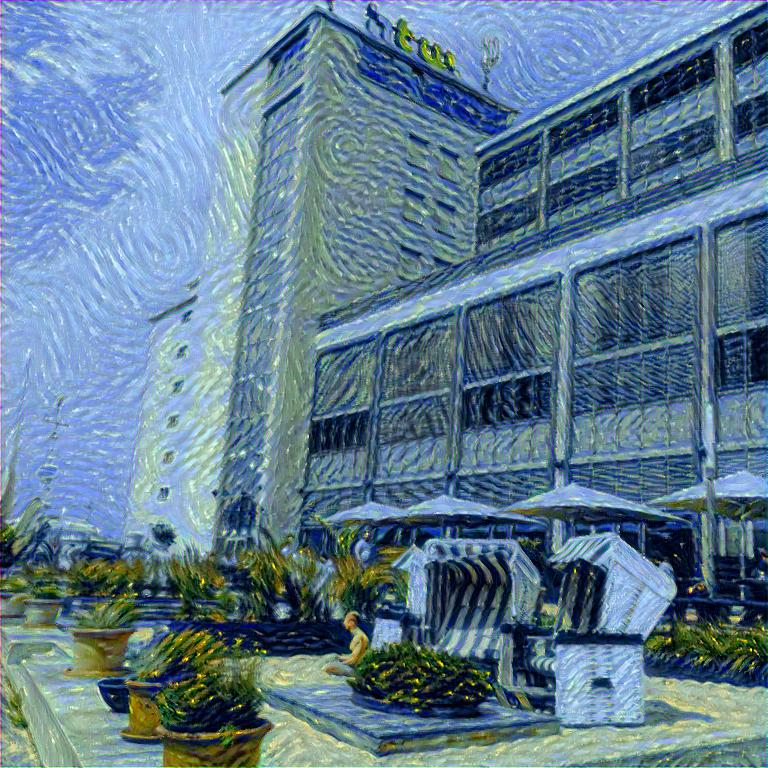
\includegraphics[width=\textwidth]{resources/content/experiments/a__starry_night__768x768__style-weight_1e+08__tv-weight_0e+00.jpg}
    \end{subfigure}
    \begin{subfigure}[h]{0.15\textwidth}
        \centering
        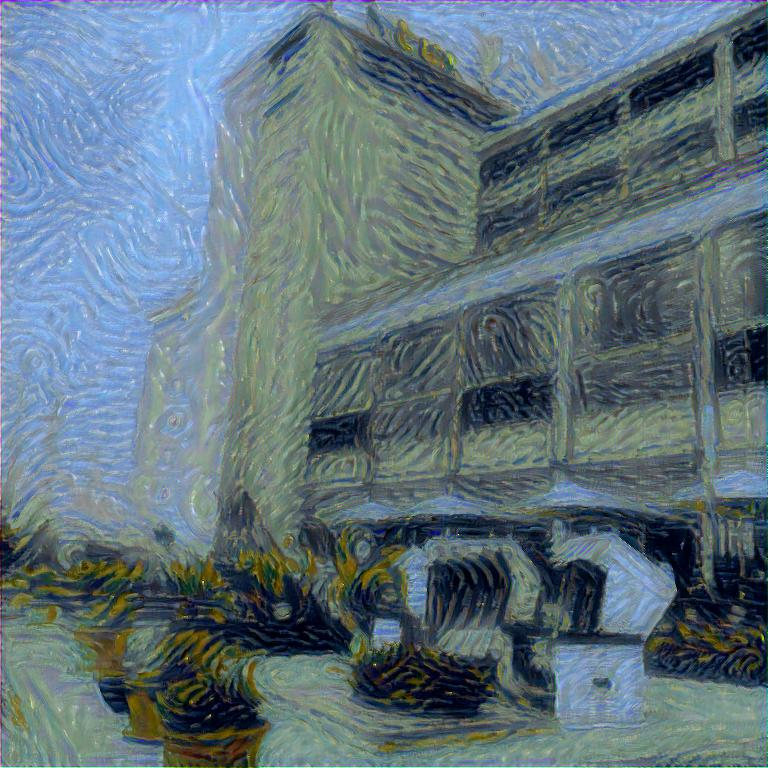
\includegraphics[width=\textwidth]{resources/content/experiments/a__starry_night__768x768__style-weight_1e+09__tv-weight_0e+00.jpg}
    \end{subfigure}
    \caption{The Starry Night mit $ \alpha = 1 $, $ \beta = 10^{5} - 10^{9} $, $ \gamma = 0 $}
\end{figure}

In der zweiten Abbildungen werden die verschiedenen Total-Variation-Gewichtungen $ \gamma = 10^{-7} $, $ \gamma = 10^{-6} $, $ \gamma = 10^{-5} $, $ \gamma = 10^{-4} $ und $ \gamma = 10^{-3} $  für Starry Night getestet.

\begin{figure}[H]
    \centering
    \begin{subfigure}[h]{0.15\textwidth}
        \centering
        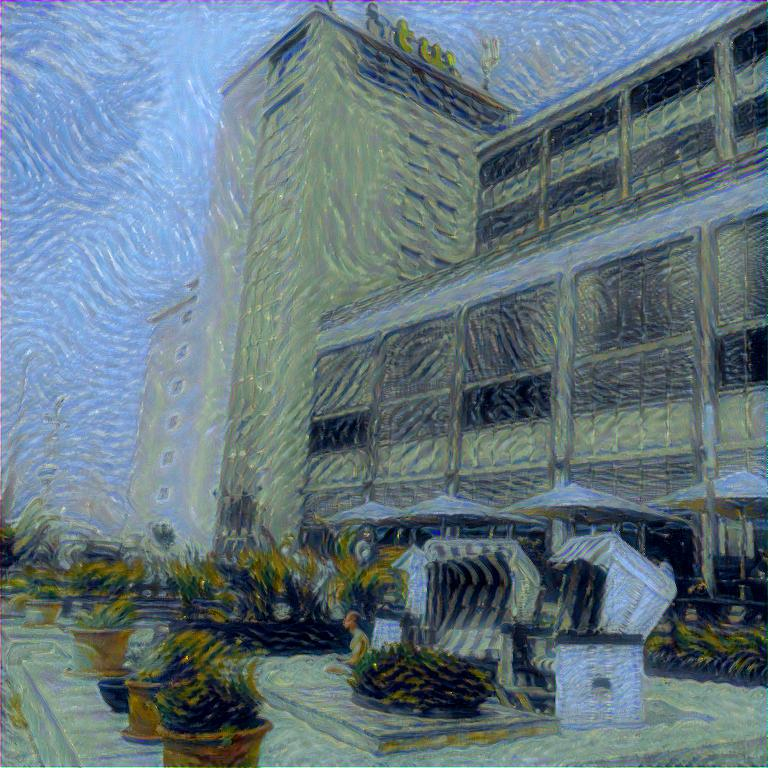
\includegraphics[width=\textwidth]{resources/content/experiments/b__starry_night__768x768__style-weight_1e+08__tv-weight_1e-07.jpg}
    \end{subfigure}
    \begin{subfigure}[h]{0.15\textwidth}
        \centering
        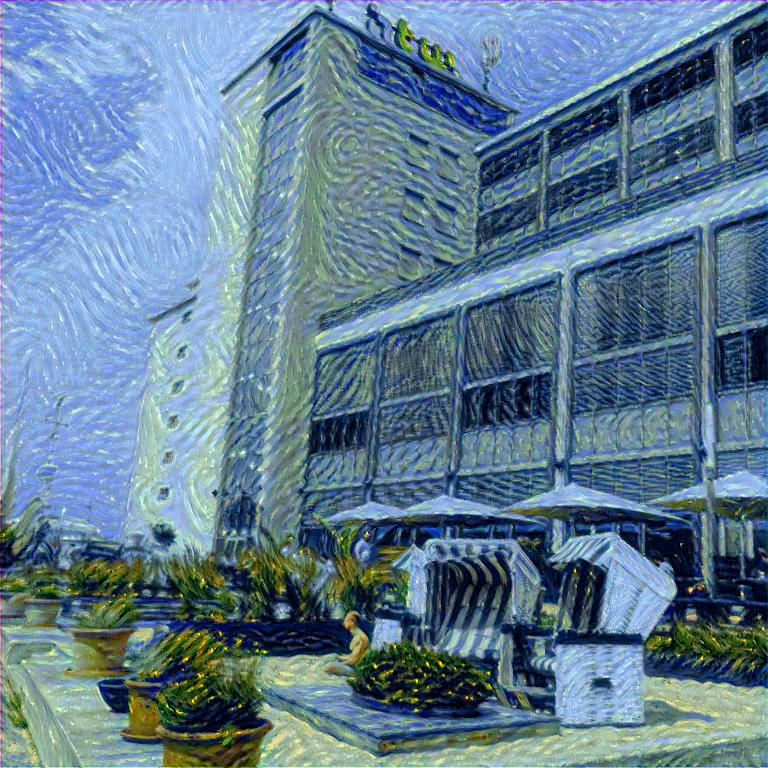
\includegraphics[width=\textwidth]{resources/content/experiments/b__starry_night__768x768__style-weight_1e+08__tv-weight_1e-06.jpg}
    \end{subfigure}
    \begin{subfigure}[h]{0.15\textwidth}
        \centering
        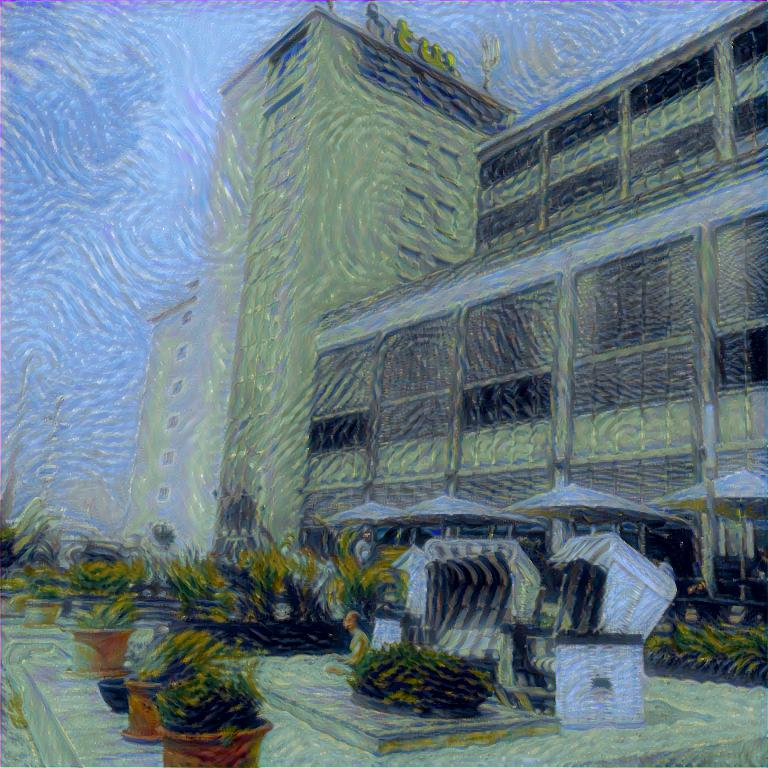
\includegraphics[width=\textwidth]{resources/content/experiments/b__starry_night__768x768__style-weight_1e+08__tv-weight_1e-05.jpg}
    \end{subfigure}
    \begin{subfigure}[h]{0.15\textwidth}
        \centering
        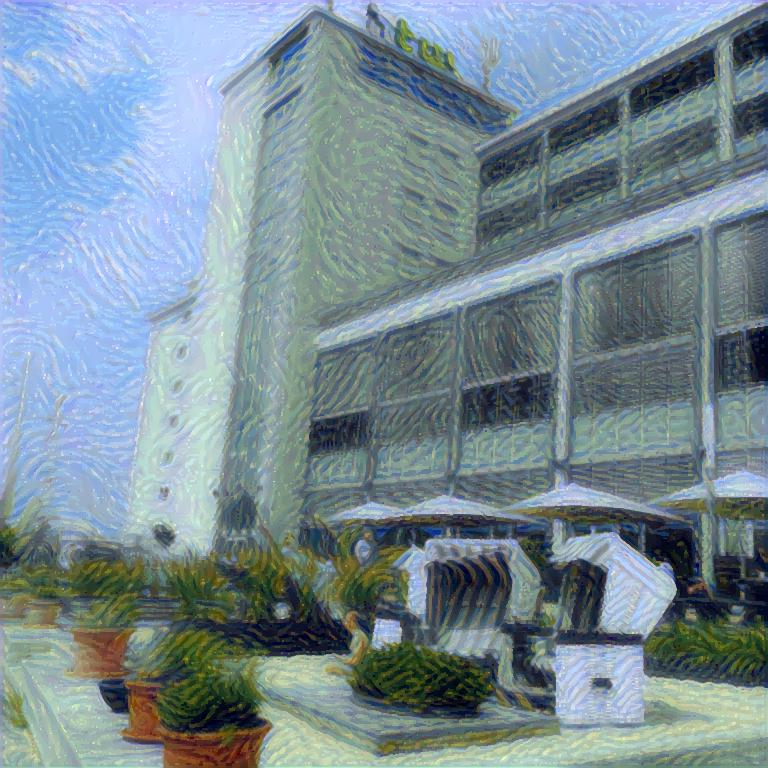
\includegraphics[width=\textwidth]{resources/content/experiments/b__starry_night__768x768__style-weight_1e+08__tv-weight_1e-04.jpg}
    \end{subfigure}
    \begin{subfigure}[h]{0.15\textwidth}
        \centering
        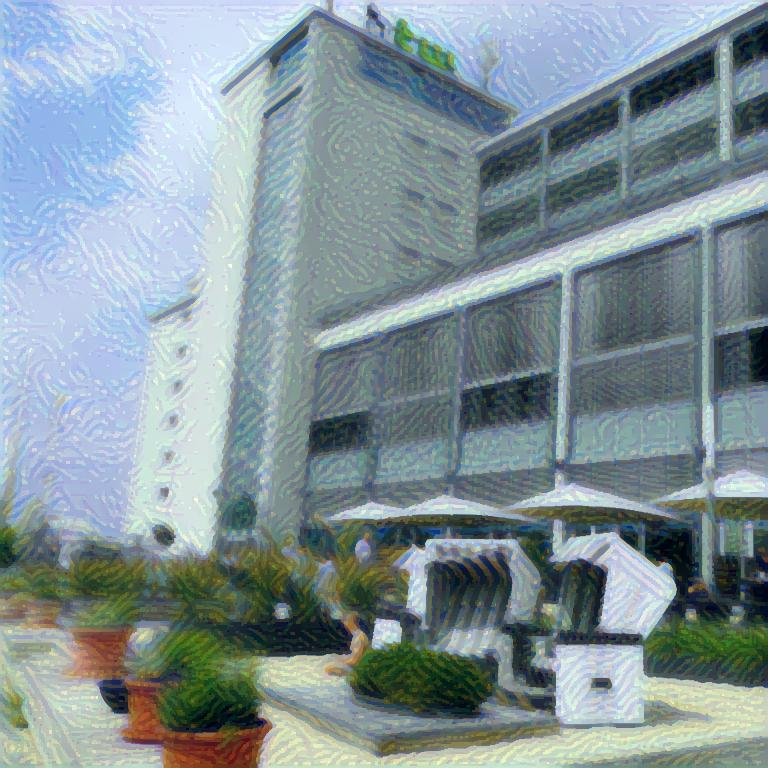
\includegraphics[width=\textwidth]{resources/content/experiments/b__starry_night__768x768__style-weight_1e+08__tv-weight_1e-03.jpg}
    \end{subfigure}
    \caption{Starry Night mit $ \alpha = 1 $, $ \beta = 10^{8} $, $ \gamma = 10^{-7} - 10^{-3} $}
\end{figure}

\pagebreak

\subsection{Experiment 2: The Scream}

\begin{figure}[H]
    \centering
    \begin{subfigure}[h]{0.20\textwidth}
        \centering
        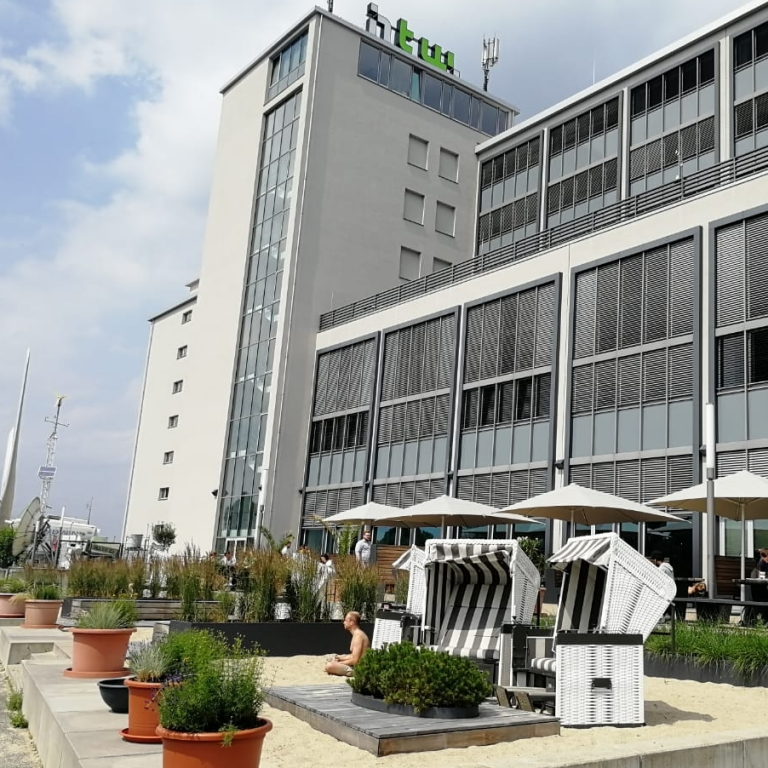
\includegraphics[width=\textwidth]{resources/content/content/htw-768x768.jpg}
    \end{subfigure}
    \begin{subfigure}[h]{0.20\textwidth}
        \centering
        \includegraphics[width=\textwidth]{resources/content/style/the_scream.jpg}
    \end{subfigure}
    \caption{HTW kombiniert mit The Scream \cite{the_scream_img}}
\end{figure}


In der ersten Abbildungen werden verschiedene die verschiedenen  \\
Stilgewichtungen $ \beta = 10^{5} $, $ \beta = 10^{6} $, $ \beta = 10^{7} $, $ \beta = 10^{8} $ und $ \beta = 10^{9} $ für The Scream getestet.

\begin{figure}[H]
    \centering
    \begin{subfigure}[h]{0.15\textwidth}
        \centering
        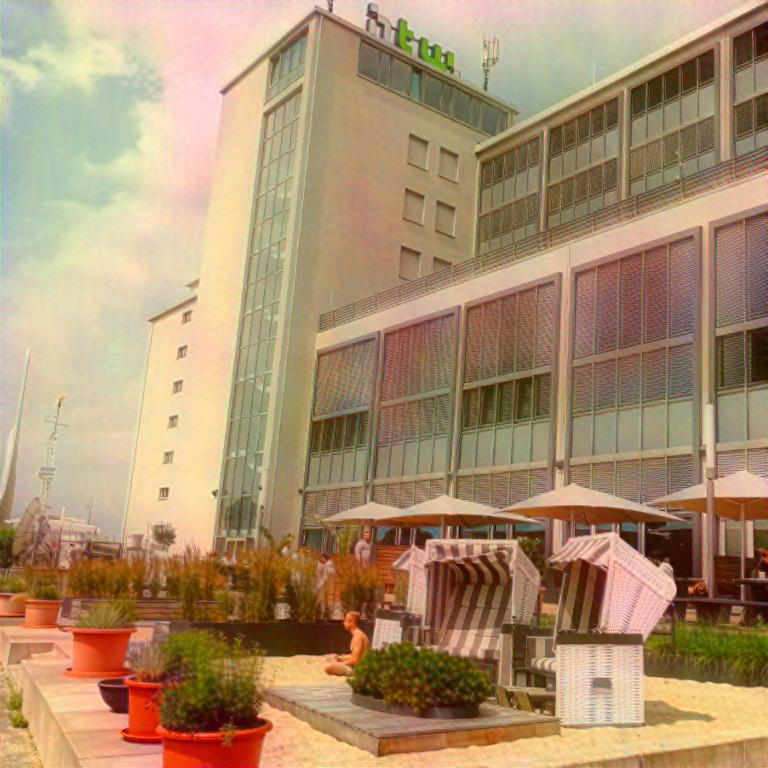
\includegraphics[width=\textwidth]{resources/content/experiments/a__the_scream__768x768__style-weight_1e+05__tv-weight_0e+00.jpg}
    \end{subfigure}
    \begin{subfigure}[h]{0.15\textwidth}
        \centering
        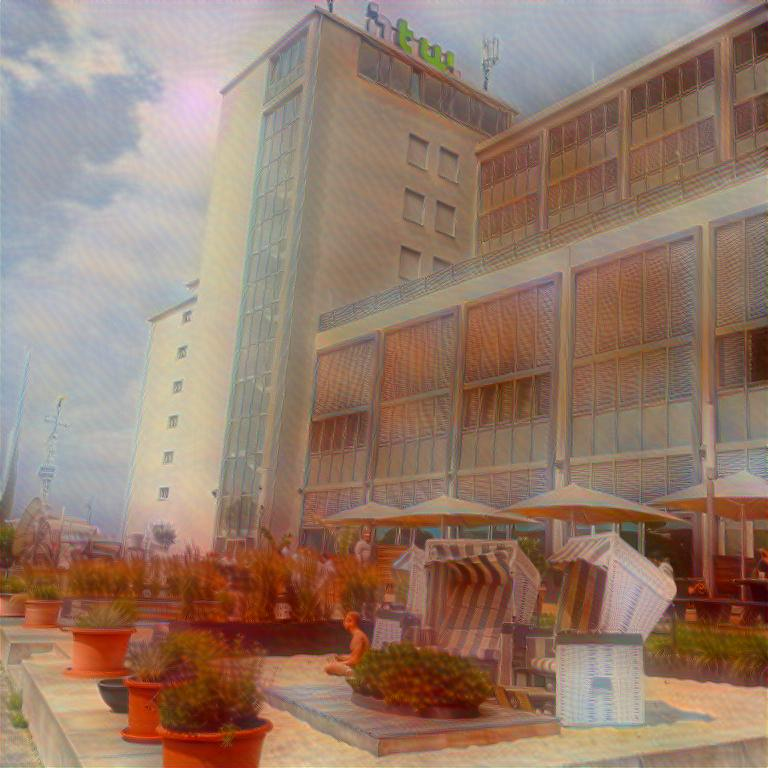
\includegraphics[width=\textwidth]{resources/content/experiments/a__the_scream__768x768__style-weight_1e+06__tv-weight_0e+00.jpg}
    \end{subfigure}
    \begin{subfigure}[h]{0.15\textwidth}
        \centering
        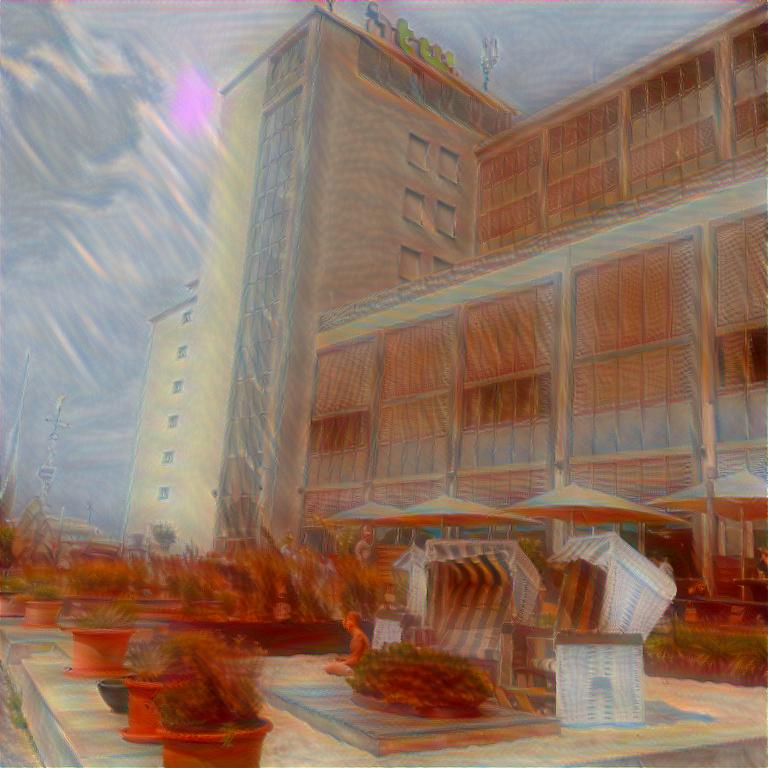
\includegraphics[width=\textwidth]{resources/content/experiments/a__the_scream__768x768__style-weight_1e+07__tv-weight_0e+00.jpg}
    \end{subfigure}
    \begin{subfigure}[h]{0.15\textwidth}
        \centering
        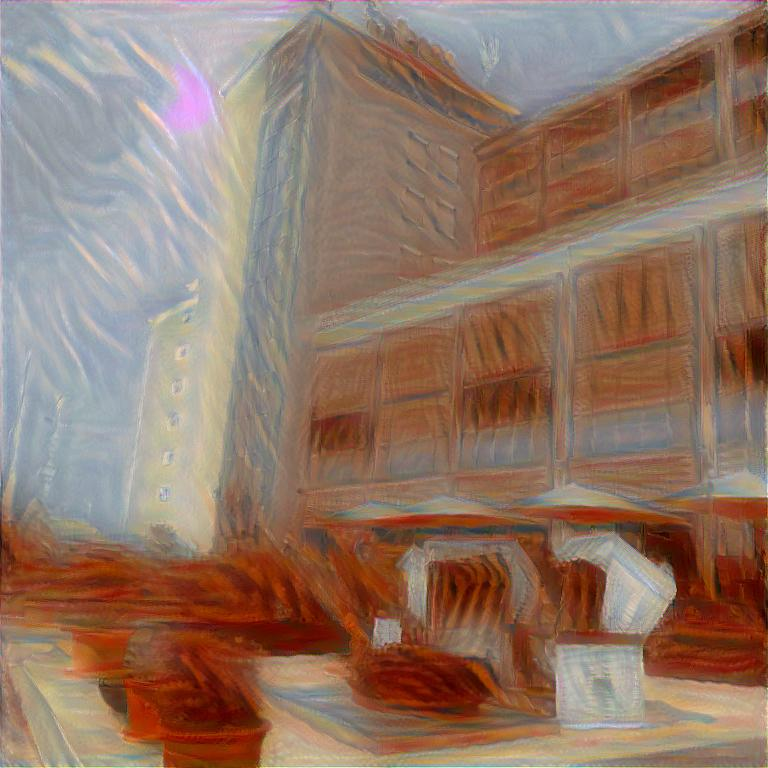
\includegraphics[width=\textwidth]{resources/content/experiments/a__the_scream__768x768__style-weight_1e+08__tv-weight_0e+00.jpg}
    \end{subfigure}
    \begin{subfigure}[h]{0.15\textwidth}
        \centering
        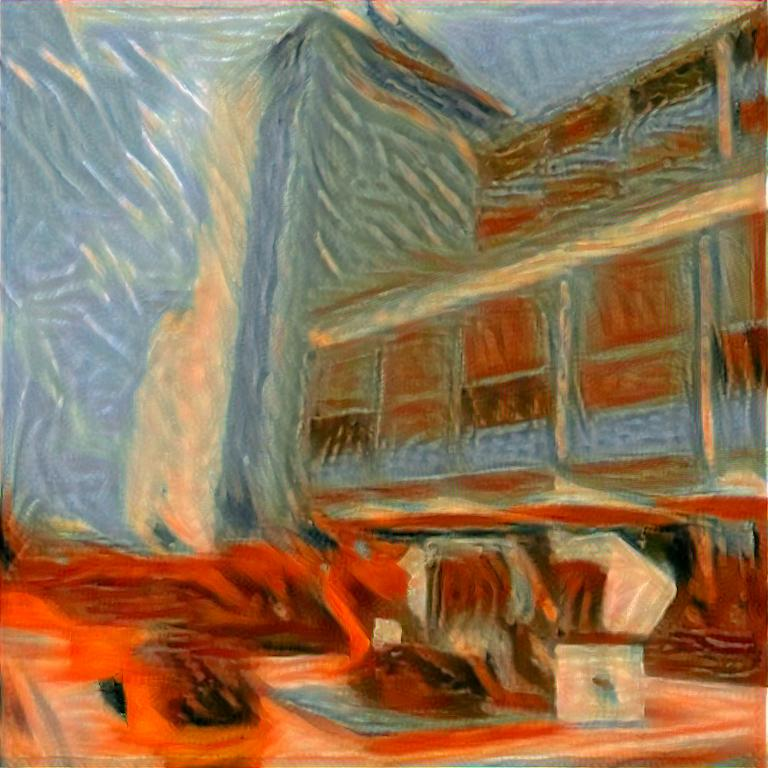
\includegraphics[width=\textwidth]{resources/content/experiments/a__the_scream__768x768__style-weight_1e+09__tv-weight_0e+00.jpg}
    \end{subfigure}
    \caption{The Scream mit $ \alpha = 1 $, $ \beta = 10^{5} - 10^{9} $, $ \gamma = 0 $}
\end{figure}

In der zweiten Abbildungen werden verschiedene die verschiedenen Total-Variation-Gewichtungen $ \gamma = 10^{-7} $, $ \gamma = 10^{-6} $, $ \gamma = 10^{-5} $, $ \gamma = 10^{-4} $ und $ \gamma = 10^{-3} $ für The Scream getestet.

\begin{figure}[H]
    \centering
    \begin{subfigure}[h]{0.15\textwidth}
        \centering
        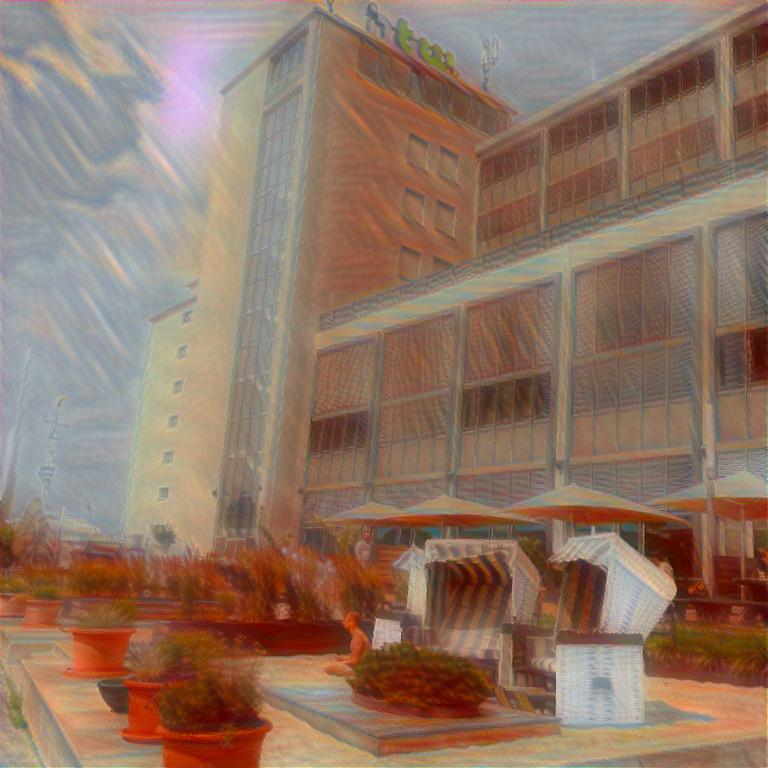
\includegraphics[width=\textwidth]{resources/content/experiments/b__the_scream__768x768__style-weight_1e+07__tv-weight_1e-07.jpg}
    \end{subfigure}
    \begin{subfigure}[h]{0.15\textwidth}
        \centering
        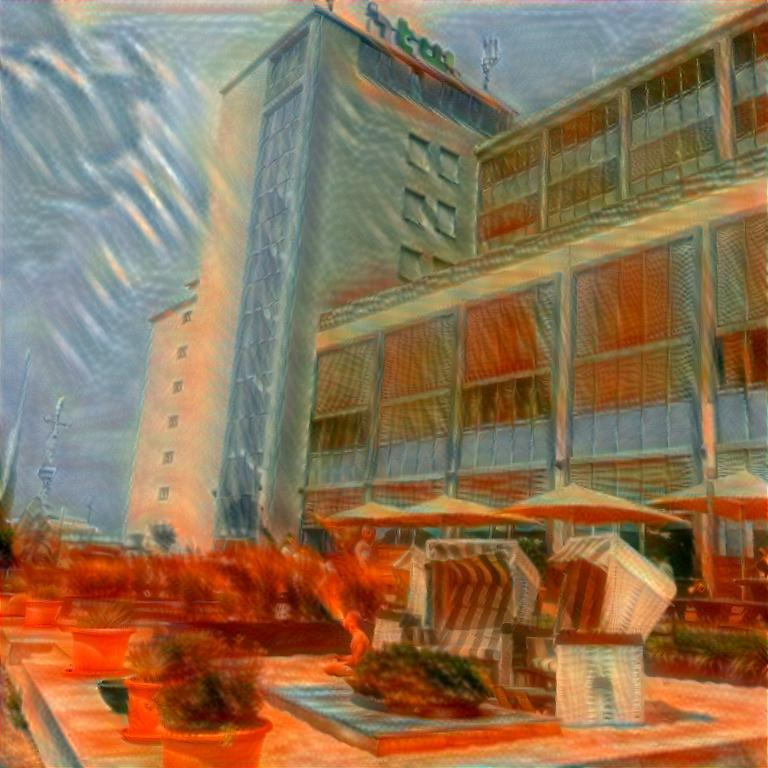
\includegraphics[width=\textwidth]{resources/content/experiments/b__the_scream__768x768__style-weight_1e+07__tv-weight_1e-06.jpg}
    \end{subfigure}
    \begin{subfigure}[h]{0.15\textwidth}
        \centering
        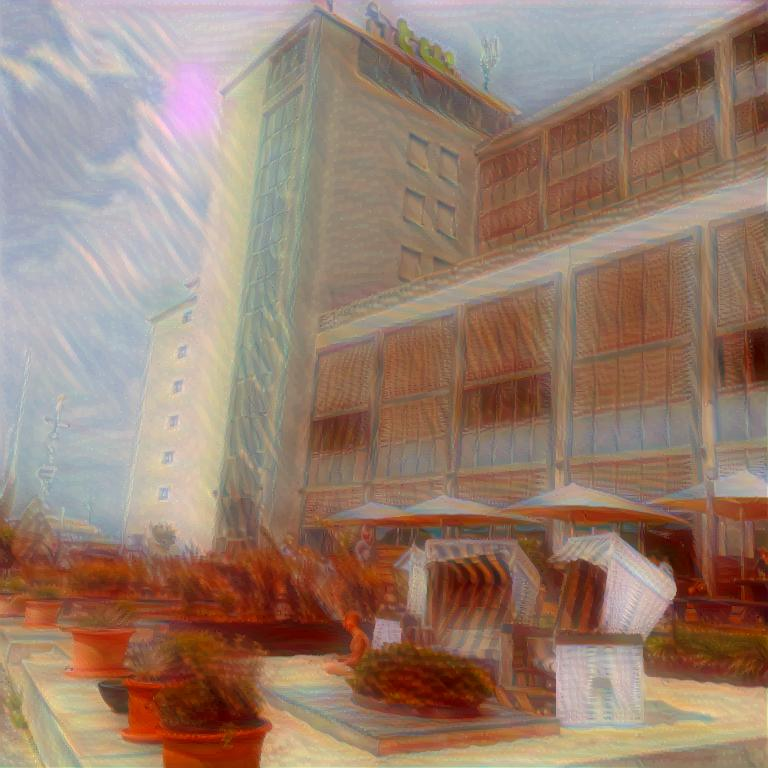
\includegraphics[width=\textwidth]{resources/content/experiments/b__the_scream__768x768__style-weight_1e+07__tv-weight_1e-05.jpg}
    \end{subfigure}
    \begin{subfigure}[h]{0.15\textwidth}
        \centering
        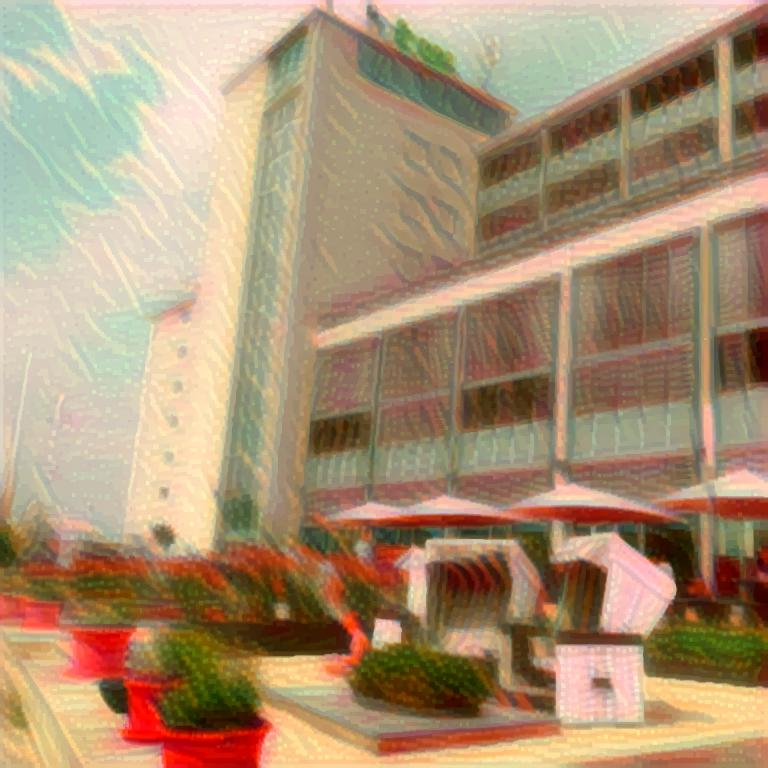
\includegraphics[width=\textwidth]{resources/content/experiments/b__the_scream__768x768__style-weight_1e+07__tv-weight_1e-04.jpg}
    \end{subfigure}
    \begin{subfigure}[h]{0.15\textwidth}
        \centering
        
\includegraphics[width=\textwidth]{resources/content/experiments/b__the_scream__768x768__style-weight_1e+07__tv-weight_1e-03.jpg}
    \end{subfigure}
    \caption{The Scream mit $ \alpha = 1 $, $ \beta = 10^{7} $, $ \gamma = 10^{-7} - 10^{-3} $}
\end{figure}

\pagebreak

\subsection{Interpretation der Ergebnisse}

Wie beiden Tests zu sehen ist, werden die Muster mit zunehmendem Style-Weight $ \beta $ auf dem Ausgangsbild immer stärker generiert. Mit $ b = 10^{5} $ sind bei beiden Stilen die Muster des Gemäldes kaum noch zu erkennen. Lediglich wird das Ausgangsbild den Farben des Stilbildes angepasst. Ein optisch ansprechender Effekt ergibt sich bei beiden Stilen ab $ \beta = 10^{7} $. 

Mit zunehmendem Total-Variation-Weight $ \gamma $ fließen die Farben mehr ineinander und das Ausgangsbild wird verschommener. Das ist besonders gut zu sehen bei The Starry Night mit $ \gamma = 10^{-3} $ und \text{The Scream} mit $ \gamma = 10^{-4} $. Für The Scream ist eine Gewichtung von $ \gamma = 10^{-3} $ bereits zu hoch gewählt. Das Ausgangsbild entwickelt sich zu einem grauen Rauschen.


\section{Auswirkungen der Netzwerkarchitekturen}

Im diesem Experiment wurden drei unterschiedlichen Bildgrößen auf unterschiedlichen Geräten auf Durchführbarkeit und Performanz getestet.
Gemessen wird die Berechnungsgeschwindigkeit beim Forward-Pass durch das Netzwerk. Ein bereits erster Indikator für die Performanz eines Neuronalen Netzwerks ist die Anzahl der lernbaren Parameter, die bei der Trainingsphase optimiert werden. Erstellt wurden 16 unterschiedliche Netzwerke mit unterschiedlichen Kombinationen für $ m $ und $ s $. 

\ref{tab:networks}

\subsection{Verwendete Geräte}

Bei der Berechnung des Forward-Pass macht es einen Unterschied ob sie auf dem CPU oder dem GPU eines Geräts durchgeführt wird. Neuronale Netzwerke können auf einer GPU schneller als auf einem CPU berechnet werden. Das liegt daran, dass eine GPU besonders auf die Berechnung von Matrix-Operationen (wie Sie auch bei grafischen Anwendungen verwendet werden) spezialisiert ist.

Die Daten werden beim Einsatz des GPUs in den Grafikspeicher geladen. Bei der Berechnung über den CPU wird der Arbeitsspeicher (RAM) des Geräts verwendet.

\subsubsection{Gerät 1: Dell XPS 15 9550}

Beim Dell XPS 15 9550 handelt es sich um einen handelsüblichen Laptop aus dem Jahr 2016.

\begin{table}[H]
    \centering
    \begin{tabular}{ |c|c| }
        \hline
        Prozessor       & Intel Core i7-6700HQ \\ \hline
        Grafikkarte     & NVIDIA® GeForce™ GTX 960M (2GB GDDR5) \\ \hline
        Arbeitsspeicher & 16GB DDR4  \\ \hline
        Festplatte      & 512GB SSD \\ \hline
    \end{tabular}
    \caption{Spezifikation: Dell XPS 15 9550}
    \label{tab:xps15}
\end{table}

\subsubsection{Gerät 2: Jetson TX2}

Beim Jetson TX2 handelt es sich um ein leistungsarmes Gerät für die Realiserung von Algorithmen der künstlichen Intelligenz auf eingebetteten Systemen.

\begin{table}[H]
    \centering
    \begin{tabular}{ |c|c| }
        \hline
        Prozessor       & Dual-Core NVIDIA Denver 2 64-Bit CPU, Quad-Core ARM®Cortex®-A57 MPCore \\ \hline
        Grafikkarte     & 256-core NVIDIA Maxwell™ GPU \\ \hline
        Arbeitsspeicher & 8GB 128-bit LPDDR4 Memory  \\ \hline
        Festplatte      & 32GB eMMC 5.1 \\ \hline
    \end{tabular}
    \caption{Spezifikation: Jetson TX2}
    \label{tab:jetson_tx1}
\end{table}

\subsection{Durchführung der Experimente}

Alle Netzwerke wurden mit einer Batch-Size von $ 24 $, Bildgrößen von 224 * 224 Pixel und einer Learning-Rate von $ 10^{-3} $ trainiert. Es wurden 6 Epochen der Trainingsdaten aus dem Jahr 2017 des COCO-Datensatzes verwendet, welche $ 118287 $ Bilder enthalten. Insgesamt wurden die Modelle mit $ 709722 $ Bildern trainiert. Dabei lag die Trainingszeit auf einem Server mit einem GeForce GTX 1080 Ti GPU pro Model zwischen 5 und 10 Stunden.

Beim Training fiel auf das die generierten Bilder großflächige, schwarze oder weiße Artefakte enthielten. Ein Austausch der finalen Aktivierungsfunktion HardTanH, vgl. \ref{sec:hardtanh}, mit der Sigmoid-Aktivierungsfunktion, vgl. \ref{sec:sigmoid}, konnte das Problem lösen.

Abschließend wurden die unterschiedlichen Netzwerkearchitekturen auf ihre Performanz getestet. Tests die wegen unzureichendem Arbeitsspeicher oder Grafikspeicher fehlschlugen, wurden als \textcolor{danger}{nicht durchführbar} gekennzeichnet. Um die Tests durchzuführen wurden Bilder der Größen 1920 * 1080 Pixel, 1024 * 786 Pixel und 640 * 480 Pixel jeweils 10 mal mit jedem Netzwerk berechnet, die Berechnugnsgeschwindigkeit gemessen, und das arithmische Mittel der 10 Durchläufe gebildet. Die Ergebnisse sind in den Anlagen \ref{tab:1920x1080}, \ref{tab:1024x768} und \ref{tab:640x480} angefügt.

\subsection{Interpretation der Ergebnisse}

Die Performanz-Tests haben ergeben, dass der Jetson TX2 mit fast allen Netzwerkarchitekturen in der Lage war den Style-Transfer durchzuführen. Für Bilder der Größe 1920 * 768  war es jedoch nicht möglich Netzwerk 1 und Netzwerk 5 zu verwenden, vlg. \ref{tab:1920x1080}. Alle anderen Netzwerkarchitekturen konnten für Full HD Bilder in weniger als einer Sekunde berechnet werden.

Die Abbildungen \ref{img:loss_the_starry_night} und \ref{img:loss_the_scream} stellen die Loss-Kurven beim Trainingsverlauf aller Netzwerke dar. Die Loss-Kurven wurden dabei mit einem laufenden arithmischen Mittel über 100 Iterationen geflächt, um die Ergebnisse besser darstellen zu können. Für beide Stilbilder ergibt sich ein ähnlicher Trainingsverlauf. Die Netzwerkarchitekturen mit mehr lernbaren Parametern erreichen ein niedrigeres Endloss. Eine Ausnahme sind dabei die Netzwerke mit dem Parameter $ m = 16 $. Sie erreichen in allen Fällen das niedrigste Endloss. In den Abbildungen sind die Loss-Kurven dieser Netzwerke mit einer stärkeren Linie gekennzeichnet.

Desweiteren wurden die optischen Ergebnisse aller Netzwerkarchitekturen getestet. Die Ergebnisse sind in \ref{img:results_the_starry_night} und \ref{img:results_the_scream} dargestellt. Wieder zeigt sich, dass Netzwerke mit dem Parameter $ m = 16 $ optisch vielfältigere Bilder generieren als die anderen Netzwerke. Daraus wird geschlussfolgert, dass die optische Vielfalt der generierten Bilder mit dem Loss zusammenhängt.

\subsection{Weitere Ergebnisse}

Auf Basis der zuvor gewonnen Erkenntniss über die unterschiedliche Netzwerkarchitekturen, wurden weitere Modelle mit unterschiedlichen Stilbildern trainiert. Für das Training wurde jeweils die Netzwerkarchitektur 2, $ m = 16 $ und $ s = 5 $, verwendet, welche in den durchführten Tests am besten abschnitt. \clearpage
\chapter{Evaluation}

Im Kapitel Evaluation werden die restlichen Kapitel dieser Arbeit beleuchtet und kritisch betrachtet. Dabei wird auf die Kapitel Grundlagen \ref{cha:fundamentals}, Methodologie \ref{cha:methodology}, Implementierung \ref{cha:implementation} und Tests und Experimente \ref{cha:tests} eingegangen.

\section{Grundlagen}

Im Kapitel Grundlagen \ref{cha:fundamentals} werden die Grundlagen von Neuronalen Netzwerken erläutert. Besonders der Backpropagation-Algorithmus \ref{sec:backpropagation} und die Beschreibung sowie tieferes Auseinandersetzen mit Convolutions \ref{sec:conv_networks} waren für das Verständniss der Problemstellung hilfreich.

Anhand der Paper von Gatys \cite{DBLP:journals/corr/GatysEB15a} und Johnson \cite{DBLP:journals/corr/JohnsonAL16} konnte die Problemstellung des Style Transfer nachvollzogen werden. Die in den Papern verwendete Loss-Funktion ist bei beiden die Gleiche. Jedoch werden unterschiedliche Notationen verwendet. Die Loss-Funktion konnte für das Trainieren eines Neuronalen Netzwerks erneut gebraucht werden. Das Paper \cite{DBLP:journals/corr/JohnsonAL16} geht jedoch nicht auf die genaue Architektur des verwendenten Netzwerks ein. Hierzu war es hilfreich die offizielle Implementierung \cite{Johnson2016} oder die Referenz-Implementierungen im PyTorch-Repository \cite{OnlineToturialNeuralStylePyTorch} zu analysieren.

Das Konzept von Total-Variation-Denoising wurde in den Referenz-Implementierungen eingebaut, ist dort jedoch unzureichend beschrieben. Eine detailierte Beschreibung ist in den Papern \cite{RUDIN1992259, DBLP:journals/corr/EstrelaMS16} vorhanden.

\section{Methodologie}

Im Kapitel \ref{cha:methodology} wurde die Vorgehensweise der geplanten Implementierung beschrieben. Das bereits in \cite{DBLP:journals/corr/JohnsonAL16} dargestellte Konzept des Image Transformer Networks wird um die Parameter der Bottleneck-Size $ s $ und Channnel-Multiplikator $ m $ erweitert. Dadurch können beliebig viele Netzwerkarchitekturen dynamisch erstellt werden und es wurde die Grundlage für weitreichende Performanz-Tests geschaffen.

Das Konzept des ResidualBlocks ist dahingehend interessant, da es auch für andere Problemstellungen verwendet werden kann. Der Effekt des \gls{vanishing_gradient} kann mit ihm bei jeglicher Art von Convolutional-Neural-Network verringert werden und ein effizientes Training der Netzwerke erleichtern.

\section{Implementierung}

Bei der Implementierung der Netzwerkarchtiktur erwies es sich als vorteilhaft, diese möglichst dynamisch aufzubauen. Die ursprünglich geplante, abschließende Aktivierungs-Funktion Hardtanh \ref{sec:hardtanh} konnte somit problemlos durch die Sigmoid-Aktivierungs-Funktion \ref{sec:sigmoid} ausgetauscht werden. Es wurde außerdem die Möglichkeit geplant, die im Bottleneck-Teil des Netzwerks verwendeten ResidualBlocks durch andere Arten von Blöcken auszutauschen.

Das in \ref{sec:method_neural_style_transfer} entworfene Skript zur Durchführung des Neural-Style-Algorithmus konnte zum Training der Netzwerke nicht wiederverwendet werden. Hierzu wurde eine Trainer-Klasse entworfen, die weitreichende Konfigurationsmöglichkeiten bietet und das aufeinanderfolgende Training mehrerer Netzwerke erleichtert.

\section{Tests und Experimente}

Im Kapitel Tests und Experimente \ref{cha:tests} wurden verschiedene Tests mit unterschiedlichen Hyperparametereinstellungen durchgeführt.
Es wurde demonstriert, wie sich verschiedene Content-, Style- und Total-Variation-Loss-Gewichtungen zueinander verhalten. Style Transfer im Allgemeinen hat weitere Hyperparameter, welche bei den durchgeführten Tests nicht berücktsichtigt wurden.

Außerdem wurden verschiedene Tests hinsichtlich der Netzwerkarchitektur und Performanz durchgeführt. Es wurde gezeigt, dass auch Netzwerkarchitekturen mit weniger lernbaren Parametern in der Lage sein können, Stile zu erlernen. Zudem wurde gezeigt, dass die gewählten Netzwerkarchitekturen größtenteils auf Geräten mit leistungsarmer Hardware zu berechnen sind.

Die im Laufe der Experimente trainierten Modelle wurden alle ohne die Verwendung des Total-Variation-Loss erstellt. Mehr Experimente könnten zukünftig die Qualität der Modelle verbessern, indem eine passende Gewichtung für das Total-Variation-Loss gefunden wird. Diese müsste für jeden Stil durch empirische Beobachtungen herausgefunden werden. \clearpage
\chapter{Fazit}

Das Kapitel Fazit beinhaltet eine kurze Zusammenfassung der Abschlussarbeit. Das Thema wird kritisch betrachtet und es wird auf mögliche Probleme eingangen.
Letzlich wird ein Ausblick über zukünfige Entwicklungen und Möglichkeiten gewährt.

\section{Zusammenfassung}

In der Abschlussarbeit wurde sich mit intensiv mit dem Style-Transfer-Algorithmen beschäftig und diese auf Geräten mit leistungsarmer Hardware getestet.
Anfangs wurde die Theorie zu Neuronalen Netzwerken und Style-Transfer analysiert. Es wurde eine Implementierung geplant und danach mit dem Framework PyTorch umgesetzt. Unterschiedliche Netzwerke wurden erfolgreich trainiert und Stile extrahiert. Verschiedene Hyperparametereinstellungen wurden getestet und die Performanz der Netzwerke gemessen.


\section{Kritischer Rückblick}

Besonders das Training und das durchführen der Experimente muss kritisch betrachtet werden. Es wurden die entsprechende Hyperparametereinstellungen nur mit zwei Gemälden getestet. Fraglich ist ob diese den gleichen Effekt bei anderen Gemälden erziehlen. Hierfür wird davon ausgegangen das für jeden Stil die Hyperparametereinstellungen erneut getestet werden müsstn.

Bei den gewählten Gemälden waren alle Netzwerkarchitekturen in der Lage den Stil zu extrahieren. Daraus kann schlussgefolgert werden das möglicherweise sogar Netzwerkarchitekturen mit weniger lernbaren Parametern, als die hier vorgeschlagenen, in der Lage sein könnte Stile aus Gemälden zu erlernen. Bei weiteren Expereminten wäre man unter Umständen in der Lage gewesen noch Performantere Netzwerkarchitekturen zu finden.

Bei der Auswahl der verwendenten Gemälde musste beim Erstellen dieser Arbeit besonders vorsichtig vorgegangen werden. Die Bilder wurden nur aus Quellen genommen die die Verwendung für Bildungszwecke erlauben. Ein kommerzieller Einsatz wäre nicht möglich. Die Verwendung von Sttyle-Transfer-Methoden wirft besondere urheberrechtliche Bedenken auf. Urheberrechtlich geschützte Bilder können dazu verwendet werden Stile zu extrahieren und auf neue Bilder zu übertragen. Die in Bezug auf Urheberrecht aufkommenden Fragen müssen für den produktiven Einsatz eine Software-Systems geklärt werden.

\section{Ausblick}

Zukünftig könnte der Algorithmen um weitere Funktionen erweitert werden. Vorstellbar ist eine Vermischung von mehrern Stilen. Hierzu müsste die das Style-Loss aus die Gram-Matrizen merherer Gemälde kombieren.

Außerdem kann eine ähnliche Methodig einen Super-Resulition-Algorithmus verwendet werden. Dieser wird ebenfalls im Paper von Johnson et al. \cite{DBLP:journals/corr/JohnsonAL16} beschrieben. Dabei muss eine Netzwerkarchitektur verwendet werden die in der Lage ist Bilder auf eine höhere Auflösung zu skalieren. Die verwendete Loss-Funktionen wäre das bereits vorgestellte Perceptual-Loss jedoch ohne den Style-Loss-Anteil.

Performanztechnisch können weitere Experimente mit kleineren Netzwerkarchitekturen durchgeführt werden. Außerdem kann der ResidualBlock durch eine andere Art von Block ersetzt werden. Die Paper \cite{DBLP:journals/corr/HowardZCKWWAA17} und \cite{DBLP:journals/corr/abs-1801-04381} behandeln sogenannte MobileNets, welche besonders auf die Verwendung von Geräten mit leistungsarmer Hardware abziehlen. Vorstellbar wäre es die verwendenten Blöcke anstelle des ResidualBlock zu verwenden und Experimente durchzufüren. \clearpage


\printnoidxglossary[title=Glossar]
\printbibliography[title={Quellen- und Literaturverzeichnis}, heading=bibintoc]

\newpage
\pagenumbering{Roman}
\appendix
\chapter{}
\addcontentsline{toc}{chapter}{Anhang A}
\section{Script Neural Style Transfer}
\label{sec:script_neural_style_transfer}
Script zur Durchführung des Neural Style Transfer Algorithmus.

\begin{listing}[H]
\begin{minted}{python}
from tqdm import tqdm, tqdm_notebook
import matplotlib.pyplot as plt
import datetime

import torch
import torch.optim as optim
import torch.nn as nn

import torchvision.models as models

from csfnst.utils import load_image, plot_image_tensor, save_image_tensor
from csfnst.utils import rename_network_layers, replace_network_layers
from csfnst.losses import PerceptualLoss
\end{minted}
\captionof{lstlisting}{Imports}
\label{lst:neural_style_transfer_1}
\end{listing}

\begin{listing}[H]
\begin{minted}{python}
output_image_file = f'...'
style_image_file = '...'
content_image_file = '...'

USE_LBFGS = False
EPOCHS = 150

force_cpu = True
use_random_noise = True
content_image_size = 200, style_image_size = 200
\end{minted}
\captionof{lstlisting}{Einstellungen}
\label{lst:neural_style_transfer_2}
\end{listing}

\begin{listing}[H]
\begin{minted}{python}
device = torch.device('cuda' if torch.cuda.is_available() and not force_cpu else 'cpu')

style_image = load_image(style_image_file, size=style_image_size, normalize=False).to(device)
content_image = load_image(content_image_file, size=content_image_size, normalize=False).to(device)

if use_random_noise:
    output_image = torch.rand(content_image.shape[0], content_image.shape[1], content_image.shape[2]).to(device)
else:
    output_image = content_image.clone().to(device)
\end{minted}
\captionof{lstlisting}{Bilder laden}
\label{lst:neural_style_transfer_3}
\end{listing}


\begin{listing}[H]
\begin{minted}{python}
loss_network = rename_network_layers(
    replace_network_layers(
        models.vgg16(pretrained=True).features.to(device).eval()[:23],
        'MaxPool2d',
        'AvgPool2d'
    )
).to(device).eval()

criterion = PerceptualLoss(
    model=loss_network,
    content_layers=['relu3_3'],
    style_layers=['relu1_2', 'relu2_2', 'relu3_3', 'relu4_3'],
    style_image=style_image,    
    content_weigth=10,
    style_weigth=1e7,
    total_variation_weigth=1e-5,
)

optimizer = optim.LBFGS([output_image]) if USE_LBFGS else optim.Adam([output_image], lr=1e-1)
\end{minted}
\captionof{lstlisting}{Loss und Optimizer}
\label{lst:neural_style_transfer_4}
\end{listing}

\pagebreak

\begin{listing}[H]
\begin{minted}{python}
content_image.unsqueeze_(0)

output_image.unsqueeze_(0)
output_image.requires_grad_()

progress_bar = tqdm_notebook(range(EPOCHS))

if USE_LBFGS:
    for epoch in progress_bar:
        def closure():
            output_image.data.clamp_(0, 1)
            optimizer.zero_grad()

            loss = criterion(output_image, content_image)
            loss.backward()

            progress_bar.set_description(f'Loss: {loss.item():,.2f}')

            return loss

        optimizer.step(closure)
else:
    for epoch in progress_bar:
        output_image.data.clamp_(0, 1)
        optimizer.zero_grad()

        loss = criterion(output_image, content_image)
        loss.backward()

        progress_bar.set_description(f'Loss: {loss.item():,.2f}')

        optimizer.step()


content_image.squeeze_()

output_image.detach_()
output_image.squeeze_()
output_image.data.clamp_(0, 1)
\end{minted}
\captionof{lstlisting}{Durchführung des Neural Style Transfer}
\label{lst:neural_style_transfer_5}
\end{listing}

\pagebreak

\begin{listing}[H]
\begin{minted}{python}
fig, axes = plt.subplots(1, 3)
fig.set_size_inches(18, 20)

plot_image_tensor(content_image, ax=axes[0])
plot_image_tensor(style_image, ax=axes[1])
plot_image_tensor(output_image, ax=axes[2])

save_image_tensor(output_image, output_image_file)
\end{minted}
\captionof{lstlisting}{Ergebnisse visualisieren}
\label{lst:neural_style_transfer_6}
\end{listing}

\pagebreak


\section{Transformer Net}
\label{sec:transformer_net_full}

\begin{listing}[H]
\begin{minted}{python}
class TransformerNet(nn.Module):
    def __init__(
            self,
            channel_multiplier=32,
            bottleneck_size=5,
            bottleneck_type=BottleneckType.RESIDUAL_BLOCK,
            expansion_factor=6,
            final_activation_fn='Hardtanh',
            intermediate_activation_fn='PReLU'
    ):
        super(TransformerNet, self).__init__()

        self.pad = nn.ReflectionPad2d(padding=20)

        self.down1 = ConvBlock(3, channel_multiplier, kernel_size=9, stride=1, activation_fn=intermediate_activation_fn)
        self.down2 = ConvBlock(channel_multiplier, channel_multiplier * 2, kernel_size=5, stride=2,
                               activation_fn=intermediate_activation_fn)
        self.down3 = ConvBlock(channel_multiplier * 2, channel_multiplier * 4, kernel_size=5, stride=2,
                               activation_fn=intermediate_activation_fn)
\end{minted}
\captionof{lstlisting}{Down-Sampling}
\label{lst:transformer_net_full_1}
\end{listing}

\pagebreak

\begin{listing}[H]
\begin{minted}{python}
if bottleneck_type == BottleneckType.RESIDUAL_BLOCK:
    self.bottleneck = nn.Sequential(*[
        ResidualBlock(channel_multiplier * 4, channel_multiplier * 4, activation_fn=intermediate_activation_fn)
        for _ in range(bottleneck_size)
    ])
elif bottleneck_type == BottleneckType.MOBILE_VERSION_ONE_BLOCK:
    self.bottleneck = nn.Sequential(*[
        MobileVersionOneBlock(channel_multiplier * 4, channel_multiplier * 4,
                              activation_fn1=intermediate_activation_fn,
                              activation_fn2=intermediate_activation_fn)
        for _ in range(bottleneck_size)
    ])
elif bottleneck_type == BottleneckType.MOBILE_VERSION_TWO_BLOCK:
    self.bottleneck = nn.Sequential(*[
        MobileVersionTwoBlock(channel_multiplier * 4, channel_multiplier * 4, expansion_factor=expansion_factor,
                              activation_fn1=intermediate_activation_fn,
                              activation_fn2=intermediate_activation_fn)
        for _ in range(bottleneck_size)
    ])
else:
    raise ValueError('Wrong value for bottleneck_type')
\end{minted}
\captionof{lstlisting}{Bottleneck}
\label{lst:transformer_net_full_2}
\end{listing}

\begin{listing}[H]
\begin{minted}{python}
self.up1 = UpSampleBlock(channel_multiplier * 4, channel_multiplier * 2, kernel_size=5, scale_factor=2,
                                 activation_fn=intermediate_activation_fn)
self.up2 = UpSampleBlock(channel_multiplier * 2, channel_multiplier, kernel_size=5, scale_factor=2,
                         activation_fn=intermediate_activation_fn)
self.up3 = ConvBlock(channel_multiplier, 3, kernel_size=9, activation_fn=final_activation_fn)
\end{minted}
\captionof{lstlisting}{Up-Sampling}
\label{lst:transformer_net_full_3}
\end{listing}

\pagebreak

\begin{listing}[H]
\begin{minted}{python}
def forward(self, x):
    x = self.pad(x)

    x = self.down1(x)
    x = self.down2(x)
    x = self.down3(x)

    x = self.bottleneck(x)

    x = self.up1(x)
    x = self.up2(x)
    x = self.up3(x)

    return x
\end{minted}
\captionof{lstlisting}{Forward-Pass}
\label{lst:transformer_net_full_4}
\end{listing}

\newpage
\pagenumbering{gobble}
\addchap*{Eigenständigkeitserklärung}

Hiermit versichere ich, dass ich die vorliegende Bachelorarbeit selbstständig und nur unter Verwendung der angegebenen Quellen und Hilfsmittel verfasst habe. Die Arbeit wurde bisher in gleicher oder ähnlicher Form keiner anderen Prüfungsbehörde vorgelegt.

\vskip 1cm

Berlin, den 20.08.2019

\vskip 1.5cm

Christoph Stach


\end{document}
